\documentclass[a4paper,11pt]{report}
%\usepackage[utf8x]{inputenc}
\usepackage[latin1]{inputenc}
\usepackage[pdftex]{graphicx}
\usepackage[cm]{fullpage}
\usepackage{subfig}
\usepackage{url}
%\usepackage{showkeys}
\usepackage{gensymb}
\usepackage{textcomp}
\usepackage{listings}
\usepackage{color}
\usepackage{appendix}
\usepackage[pdftex]{graphicx}

\newcommand{\HRule}{\rule{\linewidth}{0.5mm}}
\renewcommand{\topfraction}{.9}
\renewcommand{\bottomfraction}{.9}
\renewcommand{\textfraction}{.1}

\graphicspath{{./}{images/}}

\begin{document}

\begin{titlepage}

\begin{center}


\includegraphics[width=18cm]{title_top.png}

\HRule \\[0.4cm]
%{ \huge \bfseries Performance Evaluation of a mini UAV LIDAR for Terrain Traversability Assessment}\\[0.4cm]
{ \huge \bfseries Construction of a mini UAV and payload to assess LIDAR performance for terrain traversability mapping}\\[0.4cm]

\HRule \\[1.5cm]

\begin{minipage}{0.4\textwidth}
\begin{flushleft} \large
\emph{Author:}\\
Paul \textsc{Cox} Intern at LAAS-CNRS, 5AE INSA Toulouse
\end{flushleft}
\end{minipage}
\begin{minipage}{0.4\textwidth}
\begin{flushright} \large
\emph{Supervisor:} \\
Bertrand \textsc{Vandeportaele}
\end{flushright}
\end{minipage}

\vfill
{\large \today}

\end{center}
\end{titlepage}

\tableofcontents
\newpage

\chapter{Introduction}

This report covers a mini UAV-based project accomplished during my 6 month intership in the RIS group at the LAAS. Apart from the Introduction and the Conclusion, the contents are grouped into four chapters: Chapter 2 gives a context of the project with regard to UAVs at the LAAS in general, Chapter 3 lays out the foundation, presenting specific details on the primary elements, Chapter 4 presents the hardware and software items I designed, built, and integrated, and Chapter 5 gives an account of how we tested them and what we observed.

\chapter{Project Background and Motivation}

This report presents the author's efforts to create the material and software necessary to put a specific sensor payload in a mini UAV, to collect its data, and to determine its feasibility in future research of traversability assessment.  As such, the report focuses on the specific implementations and includes practical discussions intended to guide the group as it attempts to broaden its use of UAVs.

\section{LAAS Robotics}

The Robotics and Interactions (RIS) group of the LAAS operates a number of robots that serve as testbeds for algorithm development and research \cite{ugvs}. These indoor and outdoor robots are primarily UGVs adapted for various tasks or needs. For example, Rackham (Figure \ref{fig:Rackham}) is equipped with a plethora of vision and proximity sensors \cite{rackham}, while Jido (Figure \ref{fig:Jido}) is outfit with a manipulator \cite{jido}, and Dala (Figure \ref{fig:Dala}) is capable of high-speed outdoor travel \cite{dala}. The group is interested in complementing its ground-based fleet with airborne vehicles. The intent is to research cooperative scenarios where the airborne vehicles provide a sensing advantage due to their unique perspective and mobility. More specifically, the group decided to include a mini UAV in this years ELROB competition attempt, and the goal of this project will be to create that UAV \cite{this}. Future research subjects will be able to use the practical tools developed as a stepping stone to more theoretical undertakings on traversability assessment.

\begin{figure}[htb]
  \centering
  \subfloat[Rackham]{\label{fig:Rackham}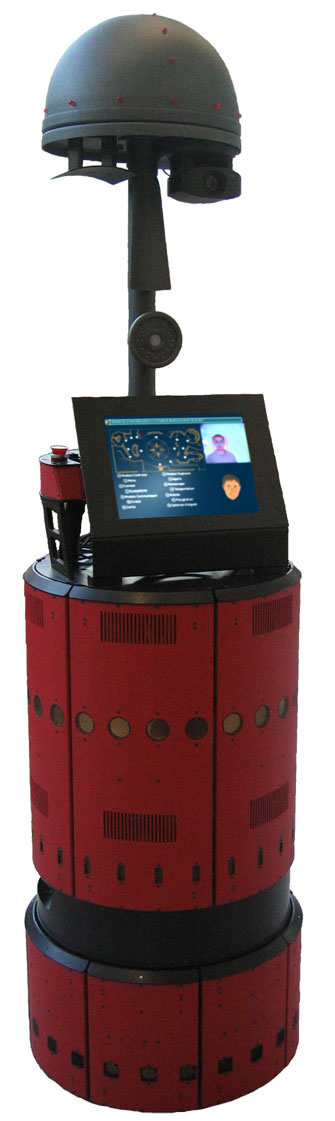
\includegraphics[width=25mm]{rackham.png}}                
  \subfloat[Jido]{\label{fig:Jido}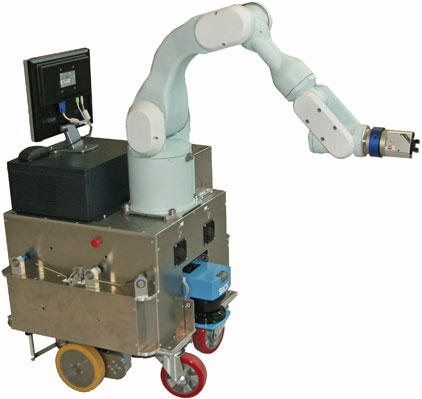
\includegraphics[width=40mm]{jido.png}}
  \subfloat[Dala]{\label{fig:Dala}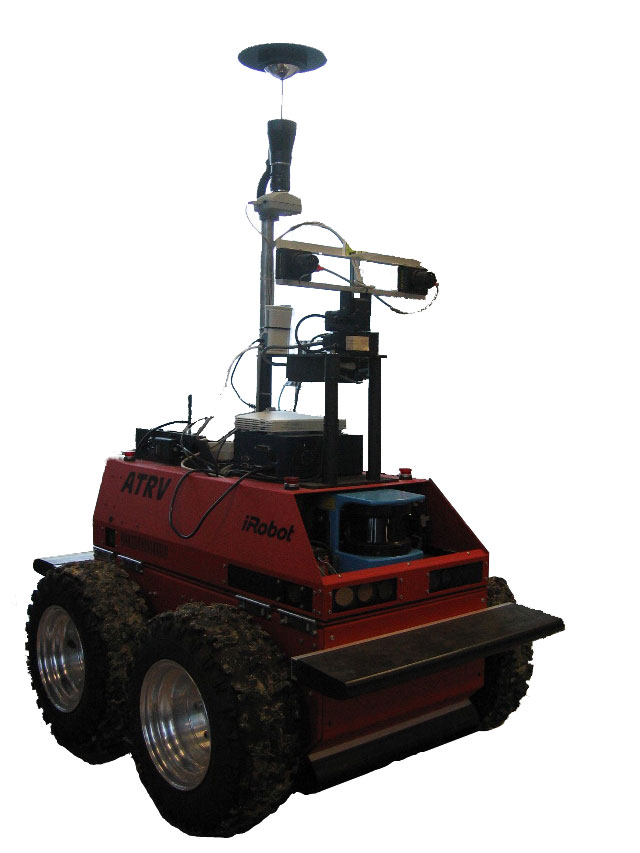
\includegraphics[width=40mm]{dala.png}}
  \caption{LAAS UGVs}
  \label{fig:ugvs}
\end{figure}

\vspace{1cm}

\section{LAAS UAVs}

There have been a number of UAV projects at LAAS: A dirigible named Karma \cite{karma}, and three fixed-wing aircraft: Lhassa \cite{lhassa}, Nirvana, and Manta. The Nirvana aircrafts were used for formation flight \cite{gautier} and not equipped with a sensing payload. Manta, a flying wing with a payload based on commodity X86 hardware, was abandoned due to it's less than convenient size and EMI issues \cite{manta}. Apart from Lhassa, these UAVs reuse the autopilot and ground station software and hardware from ENAC's open-source UAV system named paparazzi \cite{paparazzi}.

\section{ELROB Competition}

The European Land Robot (ELROB) competition is held yearly in Belgium, and the theme alternates every year between military and civilian \cite{elrob}. For the 2011 civilian event to be held in June, the competition is divided into four scenarios, namely: Reconnaissance and surveillance, Transport, Camp security, and Autonomous navigation. The primary team goal for our UAV in the competition is to assist the UGV by furnishing traversability information that will aid in the path planning process. The time to reach various waypoints is limited, so traversability data of the terrain beyond the reaches of the UGV sensors could a potential source for route optimizations.

\chapter{Project Description}

Before the project started, specific sensors and a computer board were selected for use by LAAS personnel. A fixed-wing airframe was also pre-selected. What remained was designing a solution that integrated all these individual components together into a working platform, putting it together, getting it flying, and testing performance. In this chapter I will first cover the reasons why these specific components were selected, shedding light on the overall configuration of the project, and will then describe the components themselves in detail.

\section{Sensor Selection}

The sensors were selected based on the fact that previous vision research that showed that aerial stereo imagery was not well suited for traversability mapping \cite{norman_paper}. A camera measures angles and not distances and the relatively small size of certain features relative to the distance of the UAV makes their detection impossible. Vision was abandoned in favor of laser telemetry as distances are measured directly and the precisions are high. Precision laser scanning devices, while not inexpensive, can be found in small and lightweight packages and not too much larger than cameras, so the switch from vision would not require growing the lab's UAV payload capabilities.

In straight-line flight, the laser scan data is confined to scan lines spaced out by a distance inversely proportional to the aircraft velocity (see Section \ref{geometry} for more details). To reduce the gaps in data and provide other benefits, we chose to fly back and forth over an area in one direction, and afterwards cover the smae area once again in a direction perpendicular with the first (see Figure \ref{fig:gridcarto} for an example). The resultant theoretically rectangular areas between the scan lines could then be analyzed using camera imagery. Ground texture could be aproximated for visually similar regions and this information would complement the terrain profiles acquired by laser. This data fusion would require tight time-synchronization and proper georeferencing of both the scanner and camera data to be accurate, but the concept was interesting enough to merit the inclusion of a camera on board the payload.

For attitude and position estimates, the new project would use a self-contained IMU (MTIG) instead of trying to use the autopilot's GPS along with custom hardware and software. The MTIG device fuses GPS and MEMS sensor readings into what is claimed as an accurate state estimate refreshed at a high frequency.

\section{Scan Flight Geometry}
\label{geometry}

The scanner is mounted so that when the aircraft is in horizontal flight, the scan plane is perpendicular to the ground and the aircraft's longitudinal axis. The scan line on the ground is defined by the flight parameters as follows:

nominal UAV flight velocity : 20-30 m/s

nominal UAV flight height AGL : 30 m (Manufacturer datasheet claims 30 to 60 m, later in flight we discover it is closer to 10 m)

Lidar sensor resolution : 1080 points over 270 deg visible (1440 points over 360 deg) @ 40Hz

ground covered distance during one revolution of scanner:
\begin{equation}
Dist_{per\_scan\_rev} = ground\_speed \times time_{per\_scan\_rev} = 20~\frac{m}{s} \times \frac{1}{40}~s = 0.5~m 
\end{equation}

For 90 \degree; interest zone :

scan line advances down ground track :

\begin{equation} 
Dist_{x}=  \frac{90}{360} \times Dist_{per\_scan\_rev} = \frac{1}{4} \times 0.5~m = 12.5~cm
\end{equation}

scan line proceeds along sensor rotation (for a 90 scan, this is twice the AGL height) :

\begin{equation} 
Dist_{y}=  2 \times AGL = 2 \times 30~m = 60~m
\end{equation}

Average Resolution (distance between scan points in the direction of the wingspan):

\begin{equation}  
\frac{ \frac{90}{360} \times 1440~pixels }{scan\_length} = 
\frac{360~pixels}{\sqrt{{Dist_x}^2+{Dist_y}^2}} \approx \frac{360~pixels}{Dist_y}= 6~ \frac{pixels}{m} = 17~cm
\end{equation}

Angle relative to track : (effect negligible relative to crab angle)
\begin{equation} Angle_{scan\_to\_track} = 90 - \tan^{-1} \frac{Dist_x}{Dist_y} = 90 - \tan^{-1} \frac{0.125}{60} = 90 - 0.119^\circ
\end{equation}

This information is sumarized in figure \ref{fig:geo1} and \ref{fig:geo2} below.

\begin{figure}[ht]
  \centering
  \subfloat[Overview]{\label{fig:geo1}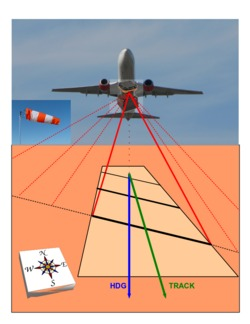
\includegraphics[width=90mm]{geo1.jpg}}                
  \subfloat[Detail]{\label{fig:geo2}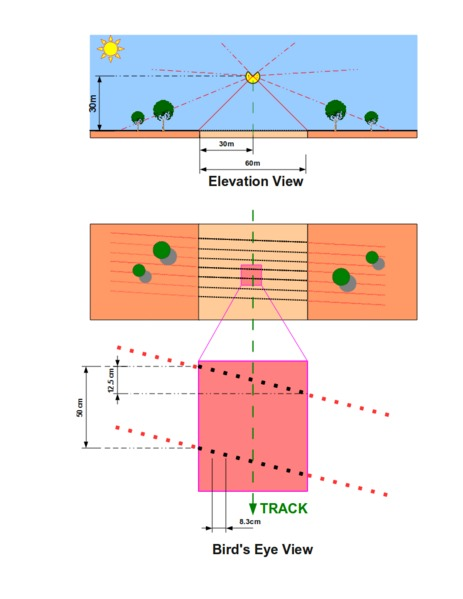
\includegraphics[width=90mm]{geo2.jpg}}
  \caption{Scan Geometry}
  \label{fig:geometry}
\end{figure}

It's important to understand that unless winds are nil, the direction an aircraft is pointing (Heading) is not the same as the direction of it's velocity vector relative to the ground it is flying over (Track). An average measure of the track can be obtained using GPS position estimates and, similarly, heading estimates using magnetometer readings, but the accuracy and precision of these estimates are quite limited when using low-cost sensors. In summary, the orientation of our airborne laser scanner will be changing constantly and practical limitations will introduce noise when the laser data is re-projected into a world frame of reference.

\section{Processor Board Selection}

The low-power ARM processor board was selected mainly to avoid the previous EMI issues of the previous project. Manta suffered from a host of issues including reduced R/C receiver range and GPS estimate corruption. These caused catastrophic crashes, and their root source was the processor board's current draw (both the amount and the quickly varying nature) and high clock frequencies of the board combined with inadequate shielding. Using a processor such as the ARM, where the entire board assembly consumes on the order of 2 to 5 Watts, significantly reduces these problems. Because of my long-running professional background with this class of processor I agreed, but was of the opinion that for a research project staying with x86 technology was less risky, especially with the recent low-power Atom offering from Intel. The reasons are that ARM System-on-Chip (SOC) processors are much more custom products than consumer grade processors, and the boards, the software, and the tools are more complicated and typically less mature. There's a big learning curve, many hidden bugs waiting to be found, and the development and integration process is much more time-consuming. An example of this is the cross-compilation nature of ARM systems. Linux cross-compliation environments are very involved technically and require extra development steps that continuously slows progress.

In short, industry uses these embedded processors for devices destined to consumer and vertical markets because of many benefits such as low per unit cost and long term availability. In a lab setting where the focus is on realizing proof of concept designs, these benefits become moot and the drawbacks are predominant.
 
\section{Payload Equipment Overview}

The computing platform selected by the group for the UAV is a low-power embedded system based on the Texas Instrument OMAP3 processor (details in Section \ref{sec:AirborneProcessor}). The Gumstix Overo module \cite{Overo}, on which the OMAP processor resides, provides the capacity to run the Linux operating system with minimal physical dimension and power requirements. 

The sensors selected include the Hokuyo UTM-30LX (Figure \ref{fig:hokuyo}), a scanning laser range finder, an XSens MTIG Inertial Navigation System (Figure  \ref{fig:mtig}), and a CMOS image sensor (Figure \ref{fig:caspa}).

\begin{figure}[htb]
  \centering
  \subfloat[Hokuyo UTM-30LX]{\label{fig:hokuyo}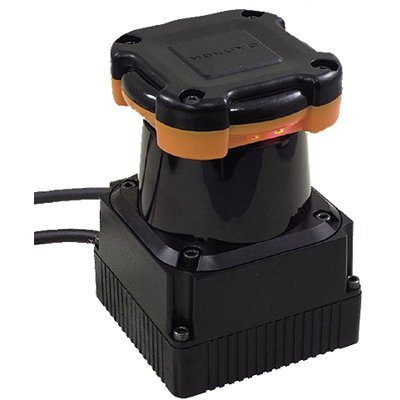
\includegraphics[width=50mm]{hokuyo.jpg}}                
  \subfloat[XSens MTI-G]{\label{fig:mtig}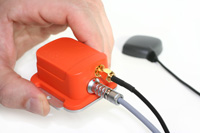
\includegraphics[width=50mm]{MTIG_inhand.jpg}}
  \subfloat[Overo and Caspa PX]{\label{fig:caspa}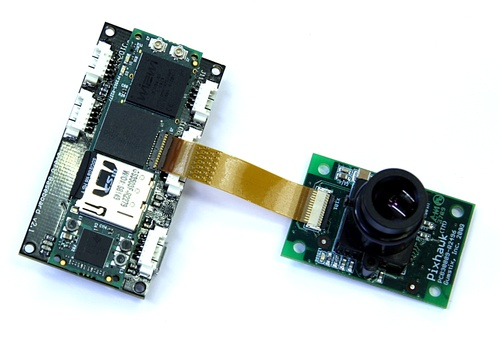
\includegraphics[width=50mm]{overo_and_caspa.jpeg}}
  \caption{Payload Primary Hardware Elements}
  \label{fig:sensors}
\end{figure}

This payload equipment will reside on-board a low-cost aircraft controlled by the paparazzi autopilot system as detailed in Sections \ref{sec:mentorproject} and \ref{sec:paparazzi}, respectively.

\subsection{Airborne Processor}
\label{sec:AirborneProcessor}

In this section we present the miniature embedded computer present on our UAV. It's purpose is to gather the sensor data, log it to disk, communicate with the ground, and eventually to perform vision and mapping-related processing.

\subsubsection{Hardware}

The central component of the payload is the Gumstix Overo module (Figure \ref{fig:overo_mod}). The module is used along with a carrier board. The carrier board selected for this project is the Summit product from Gumstix (Figure \ref{fig:overo_summit}). Together, the module and the carrier board contain the TI OMAP processor along with wifi, ethernet, bluetooth transceivers, and a convenient micro SD socket. The TI OMAP System On Chip (SOC) processor incorporates a 600MHz 32-bit ARM Cortex-A8 core, a DSP, and many peripherals including UART, I2C, SPI, SD, USB, and a dedicated camera interface. The package-on-package (POP) configuration, where the SDRAM and NAND memory are stacked directly on top of the processor saves valuable space and weight and decreases EMI/EMC issues. While the camera interface and the DSP provide for future research capabilities, in the near term the important interface is USB Host as this will be used to receive laser scanner data along with other serial-based communications (Inertial Navigation System, ground communication modem, and autopilot communication).

\begin{figure}[htb]
  \centering
  \subfloat[Overo Module]{\label{fig:overo_mod}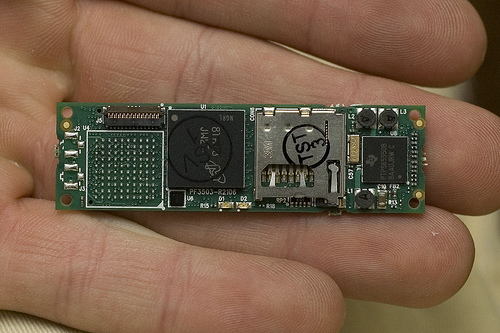
\includegraphics[width=80mm]{overo_in_hand.jpg}}                
  \subfloat[Module on Summit carrier board]{\label{fig:overo_summit}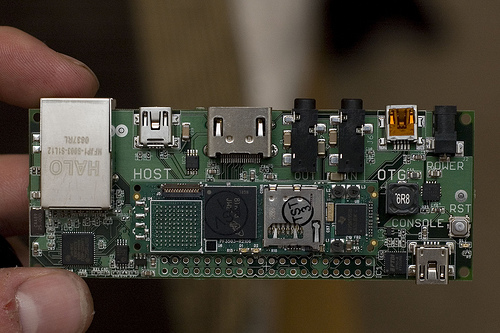
\includegraphics[width=80mm]{overo_on_summit.jpg}}
  \caption{Gumstix Overo}
  \label{fig:overo}
\end{figure}


\subsubsection{Software}

The OMAP processor runs a full Linux operating system, cross compiled on a standard Linux host using a compilation system called OpenEmbedded. OE is capable of generating the necessary bootloader, linux kernel and modules, along with a root file system populated with all of the libraries and applications that might be needed to run our payload code. Configuration is done using bitbake recipes. With assistance from LAAS developers, bitbake recipes are available for the hokuyo and MTIG device libraries on the OMAP3 plaftorm. These libraries are compiled into ipkg packages that can be installed on the target using the opkg command. Our own custom C++ application links to these libraries and performs all of the acquisition and logging activities. The application is compiled using the paparazzi omap toolchain using a makefile integrated into the paparazzi build environment.

What is important to appreciate is that the cross-compilation environment is extremely complex and development takes considerable time. Many system administration and development skills are a prerequisite to make progress with them. Setting up and using the configuration and build tools, building Linux kernels and drivers, creating bootable disks with the proper programs and partitions; all these tasks require a newbie many days each to first understand and then learn to apply. And when there's bugs or things just don't work as they should, a lot of time must be dedicated to digging in depth and learning the nitty-gritty details hidden in the layers below.

The Makefile and source code are available in Appendix B.

\subsection{Airborne Sensors}

This section details the miniature sensors carried aloft by our UAV. These include a laser scanner, a camera, and an Inertial Navigation System.

\subsubsection{Hokuyo UTM-30LX}
\label{Hokuyo}

The UTM-30LX scans a single line around it's central axis at a maximum rate of 40 Hz. A distance and reflectivity measurement is taken at a resolution of 1/4 of a degree, it's field of vision is 270 degrees, and distance resolution is in the millimeter range. The USB interface, along with open-source software drivers \cite{robotpkg}, allows interfacing to PC and embedded hosts, but as we discovered later in the project (and detailed in Section \ref{hokuyo_perf}) a number of practical limitations cause the actual maximum data rate to be considerably below what is expected, and the range is significantly below the 30 to 60 meters claimed in the manufacturer datasheet.

\subsubsection{Aptina MT9V032 Camera}
\label{caspa}

The MT9V032 CMOS device from Aptina was selected due to its global shutter characteristic that guarantees that all pixels in a frame are acquired simultaneously (unlike the much more common rolling shutter cameras found in most webcams, cell phones, etc). This is a very important feature if the camera is moving or rotating. Camera resolution is 752 x 480 pixels and is available in color or black and white. 

The CMOS Camera is interfaced to the OMAP processor using the dedicated camera bus by means of level converters (1.8V/3.3V) and a high-density flat flex cable. This direct connection is a parallel bus with a maximum clock rate of 40MHz, which allows for fast and efficient acquisition of image data. A custom designed camera board using this sensor is in the works at the LAAS. A couple of weeks of my time was spent looking into the camera interface specifications and their compatibility with the OMAP3 and OMAP4 processor camera peripherals known as the ISP (Image Signal Processor). Beyond just recuperating the camera pixels, the ISP is a hardware peripheral capable of performing basic functions such as color conversion and image resizing. I assisted in the schematic design of the LAAS board which gives external access to the sensors exposure trigger. Initial testing for this project however depended on the commercially available camera board from Gumstix, INC called Caspa Px \cite{caspa}, and displayed in Figure \ref{fig:caspa}.

Software support is provided as a linux driver, currently for kernel version 2.6.34. The driver has been tested in flight (samples available in Figure \ref{fig:caspa_sample}) and final image quality and frame rate performance remains to be determined. It is already apparent that the driver source code is not mature or well structured. For example, color space conversions are non-standard and buggy, and more limitations are sure to be found with continued investigation.

\subsubsection{XSens MTIG INS}
\label{MTIG}

The XSens MTIG device uses MEMS sensors along with a GPS receiver to generate attitude and position estimates at a maximum rate of 120Hz using an undocumented Kalman filter running on its embedded processor. It is optionally capable of providing raw sensor measurements at a rate up to 500Hz. The serial interface is well documented and supported with various open-source libraries including LAAS' robotpkg \cite{robotpkg}. What we'll discover later is that the baudrate limits our refresh rate considerably and other issues with the device driver software will require considerable development time to identify and resolve.

While the terms INS (Inertial Navigation System), IMU (Inertial Measurement Unit), and AHRS (Attitude and Heading Reference System) are usually non-overlapping terms, in this document their use are synonymous.

\section{Autopilot System}
\label{sec:paparazzi}

In this section we cover the background information on the open-source UAV platform known as paparazzi. We use this platform in our project to gain a mature autopilot and a ground station.

\subsection{Paparazzi Overview}

Paparazzi is an autopilot system based on a C-code mainloop program running on an airborne ARM microcontroller and Ocaml ground-station code running on a standard Linux PC or laptop \cite{paparazzi}. The autopilot board is called the Tiny (Figure \ref{fig:tiny}). The system allows for extensive customization and extensions. For example, the flight plan mechanism allows the creation of complex trajectories based on waypoints and conditions. Some other options include support for multiple simultaneous aircraft and ground stations,  a software bus model that makes the creation and insertion of additional software agents into the system straightforward, and various simulation capabilities that are useful in initial testing of code and configurations. Ground to air communications are typically achieved with low-bandwidth serial modems and commercial R/C control receivers and transmitters. 

\subsection{Aircraft Types}

Paparazzi supports fixed-wing and rotating-wing aircraft. There is much recent use of quadrotor platforms, especially the Asctec airframe \cite{asctec}, but helicopter use has so far been very limited. Users of the fixed-wing configuration typically use small foam airframes such as the ones manufactured by RC manufacturer Mutliplex \cite{multiplex}, brushless electric motors, and the wingspans remain below 1.5m. In a few cases, the airframes are much larger, or much smaller, or more complex. These might incorporate fiberglass or carbon airframes for extended runtime \cite{murat} or range \cite{corsica}, or a gas turbine to achieve higher velocities, or larger wing areas and increased payload capacity. Essentially, the PID algorithms implemented in paparazzi are such that just about any standard craft can be controlled if the gains are adjusted properly.

In the most basic and most widely used fixed-wing configuration, the autopilot uses GPS and IR sensors for attitude and navigational control \cite{paparazzi_paper}. Due to some of the drawbacks of these sensors, support for replacement or complimentary sensors exists and is continuously explored. This includes the use of static and dynamic pressure sensing (to allow the aircraft to respect air-speed or altitude bounds or set-points, for example), the use of inertial measurement units (to eliminate the need for a minimum ground/sky IR contrast, for example), and the use of a magnetometer to obtain a measure of the aircraft's heading. To maintain an accurate state estimate with small craft capable of high roll rates, the bandwidth-limited IR sensors are complemented with a roll gyro. This is typically a low-cost MEMS sensor, of the likes from Analog Devices, and interfaced via the autopilot's extra digital interfaces or sampled by an ADC channel.

\subsection{Hardware}

The current autopilot hardware is the Tiny2.1, a 50-gram board with a NXP LPC2148 microcontroller, a U-blox GPS receiver module and antenna, and small Molex Picoblade connectors for interfacing with the following devices :

\begin{itemize}
\item UART-based modem (typically Digi XBee/XBee Pro, or Aerocomm)
\item PPM-based RC receiver input (PPM signal output requires receiver modification)
\item PWM-based RC servo outputs
\item USB for programming by PC Host
\item ADC inputs to sample IR sensors and monitor battery level
\item I2C and SPI interfaces for additional communication, sensor, or actuator options (see examples cited above)
\end{itemize}

\subsection{Tradeoffs}

A typical useful hardware and software system must wrestle with the complexity trade-off. Either designs follow the KISS principle, and favor lightweight and easy to master architectures, or they aim to deliver a high degree of modularity and configurability to enable extensibility, continuous reuse and evolution. Paparazzi adopts the KISS principle for hardware designs, choosing to use COTS modules and skipping any redundancy, subscribing to the idea that a simple, straightforward, clean, and well-documented design can be relatively robust and enables a larger community (for many, a hobby activity). The software side is very different because extensibility and configurability were goals from the outset and development has continuously evolved without any milestones or official releases. This has resulted in a complex and sparsely documented code base that can seem unwieldy to anyone except a dedicated developer with the proper amount of pre-requisite competencies.

Like all active complex configurable systems, the challenge with paparazzi is its steep learning curve and rapid and continuous evolution. Tailoring the system for a specific application is not difficult because paparazzi requires extensive modifications, but because much of the system has to be mastered before a clear idea emerges of how and where the modifications should be made. Since documentation is limited to unstructured wiki pages and due to a complete lack in code comments, a user is essentially forced to become a developer and to dive deep into the system or resort to hacks to limit the time invested. Beyond the obvious drawbacks of the later option, is the fact that such hacks are only useful in the very short-term. Since the hacks will not be able to be merged with the software base, as the base evolves the hacks will continuously break and require constant effort to keep them working. This pressure is the reason why many users have forked the paparazzi code, added their extensive application-specific modifications without staying up to date, to end up with a system that is nearly un-mergeable with the evolved paparazzi code base. The bottom-line is that tailoring paparazzi for a project should be approached in one of two ways depending on the objectives. One, if the intent is to produce a one-off demo and future reuse is not a consideration, a fork can be considered along with quick hacks. If the continuous evolution of the application is envisioned or if sharing the capabilities with other paparazzi users is desired, the time to properly integrate customizations and continuously maintain them needs to be anticipated and allocated. This is the same sort of commitment already in place for the LAAS' openrobots software.

All this to say that considerable time is required to integrate paparazzi into any project and that new team members will not able to contribute for the few months it takes to get to know the system. I started using paparazzi since 2008 so had a head-start and we were fortunate to have access to the developers during the project. They were gracious enough to educate and help us throughout the project and without their assistance our efforts would have been considerably less advanced.

\chapter{Construction}

This chapter recounts the efforts in the building of the hardware and software detailed previously. We first devised a simple ground test to get some practical experience with the sensors and to start building the application software to treat the data streams. The construction then focused on putting together an autonomous plane together and the lengthy construction of a streamlined payload to house all of our expensive electronics.

\section{Payload Equipment Ground Tests}

In an attempt to gain some practical experience, flesh out any early limitations, and begin developing data processing software, a simple ground-based test was carried out. This section focuses on these initial investigations.

\subsection{Description}

While I was in the process of building the aircraft, I developed a mobile test bench. I mount the hokuyo sensor along with the MTIG to an aluminum boom and attached it to a standard bicycle as show in Figure \ref{fig:bike}. 

\begin{figure}[ht]
 \centering
 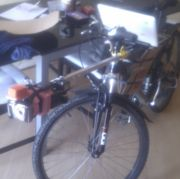
\includegraphics[width=6cm]{Bikesciencepackage.jpg}
 \caption{Bike Test Vehicle}
 \label{fig:bike}
\end{figure}

While the bicycle traveled through a residential neighborhood, a small laptop logged the sensor data to files. By analyzing the data afterwards using custom software, the logs showed that at these low speeds the sensors were providing accurate attitude, position, and laser telemetry data. They also showed that on a sunny day the hokuyo can detect a light-colored surface, perpendicular to the ray of laser light, up to aproximately 20 meters. UAV testing (discussed later in Section \ref{flight_tests}) will later show that performance on surfaces such as dirt and grass and at angles approaching 30 to 45 degrees from perpendicular is much reduced.

\subsection{Output Sample}

Using a number of PERL programs I developed (Appendix B), a composite image is generated including a number of text data such as the MTIG output angles and a graphical representations of laser scan data, the location data, and video taken by the boom mounted digital camera (Figure \ref{fig:plotlogsample}). The images are then put together to create an animation showing the entire path. The hokuyo data was recorded at a rate of approximately 20 Hz while the MTIG Data was near 100Hz. Rough synchronization is accomplished by using the MTIG data sample with a timestamp closest to the one in a laser scan (each laser scan is also timestamped). Later we would discover that the timestamps were not correct due to device driver issues but we did not catch it here as the bicycle was moving quite slowly.

\begin{figure}[ht]
 \centering
 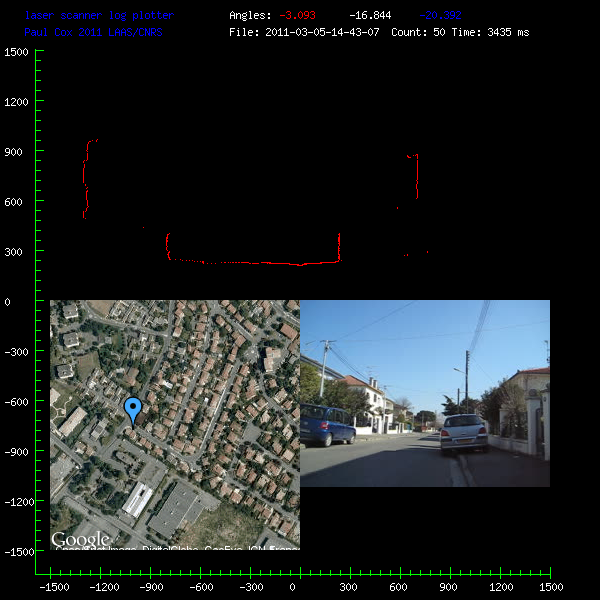
\includegraphics[width=12cm]{Plotlogsample.png}
 \caption{Sample animation frame}
 \label{fig:plotlogsample}
\end{figure}

Ground testing showed the hokuyo device can be used in an exterior setting and that distances of up to 16 meters can be detected even in bright sunlight if the reflecting surface is perpendicular and of a light color.

\subsection{3D Terrain Modeling}

The next step intended step was to represent the laser scans in a 3D environment, creating a Digital Terrain Model and representing it graphically in an openGL tool such as GDHE. This process can be accomplished with the LAAS tools, but this is complex and mostly undocumented software devoid of tutorials. I am still trying to learn these so this tasks is not yet complete. At the request of my advisor and to become familiar with methods behind these sorts of tools, I developed a number of software applications. The code is available freely online \cite{laserhawkgit}. Some screenshots of these applications are shown below in Figure \ref{fig:mkvirt} and \ref{fig:hoku2gdhe}.

\subsubsection{Virtual Terrain Generation}

Using the PERL language, I created software that could create sensor logs using a virtual environment. The environment includes a bounded surface that defines the terrain topography and camera orientation. The model can be defined as piece-wise functions or by a greyscale bitmap. An example terrain is shown in Figure \ref{fig:mkvirt}. Lighter colored pixels have higher elevation than darker ones. In this specific example, the scanner is 7 m above the surface and angled at 35 degrees from vertical. The top set of red scan lines are part of an elevation view of the scense. The scan lines stop at their intersection with the surface. The bottom set of red scan lines are a top or ``bird's eye'' view of the scene, and the 35 degree scanner angle is apparent as the rays are stricking the surface at an angle. Graduation marks on the edges are in centimeters.

\begin{figure}[ht]
 \centering
 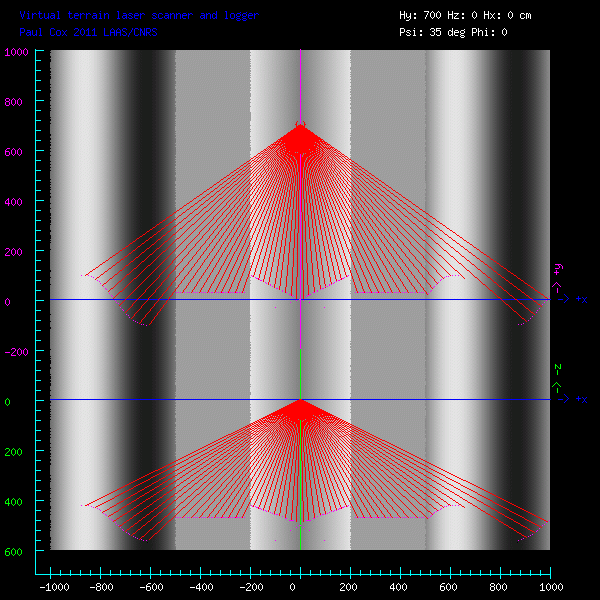
\includegraphics[width=12cm]{Mkvirtsample.png}
 % Mkvirtsample.png: 0x0 pixel, 300dpi, 0.00x0.00 cm, bb=
 \caption{Virtual terrain simulator}
 \label{fig:mkvirt}
\end{figure}

The virtual terrain surface is ``scanned'' along a line by using a raycasting method. Essentially, iterating through the scan angles one step of resolution at a time, the distance between the scanner and the surface is calculated. The calculation is performed by propagating the ray until intersection is detected, and uses some trigonometry to arrive at a final distance.

After acquisition of the virtual scan lines into log files, 3D plotting tools can be used to visualize them (see following section).

\subsubsection{3D Plots of Terrain Data}

Using an MTI IMU and a hokuyo scanner, we developed a C program that could be used to reconstruct a scene in 3D. The scan data is rotated into a world reference frame using the IMU data and then displayed in GDHE. Figure \ref{fig:hoku2gdhe} shows the program in use while the device is in my living room.

\begin{figure}[ht]
 \centering
 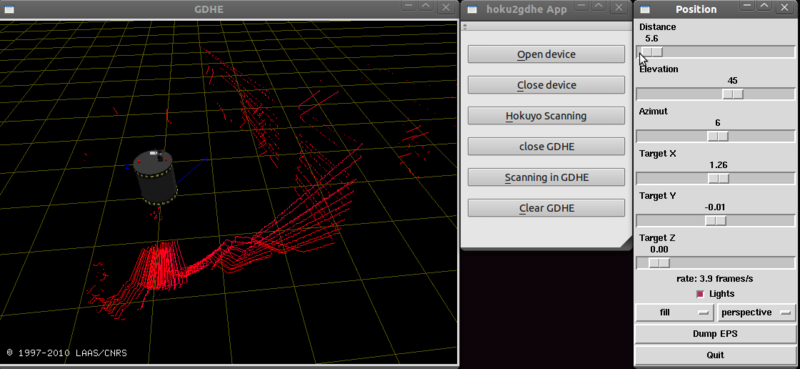
\includegraphics[width=18cm]{Hoku2gdhe.png}
 % Hoku2gdhe.png: 0x0 pixel, 300dpi, 0.00x0.00 cm, bb=
 \caption{Data visualisation in GDHE}
 \label{fig:hoku2gdhe}
\end{figure}


\section{Mentor Aircraft}
\label{sec:mentorproject}

As explained in the introduction, the primary short-term goal was to outfit a Multiplex Mentor aircraft with a Hokuyo scanner, a Gumstix Overo, a camera, and an MTIG for the June 2011 competition. Towards this goal, I've integrated a paparazzi autopilot in a standard Mentor airframe, doing all of the cabling and other tasks myself. I've also built a reinforced modular payload pod to hold the science package in an easy removable format. The removable pod design permits development with the science package in a lab or office environment without being encumbered by the airplane, and provides some level of protection to the sensitive electronics in the event of a crash.

\subsection{Airframe}

The aircraft is a standard three-axis electric R/C model and is displayed in Figure \ref{fig:mentor}. It uses two ailerons, an elevator, and a rudder for control surfaces along with a fourth channel for thrust control.

\begin{figure}[ht]
 \centering
 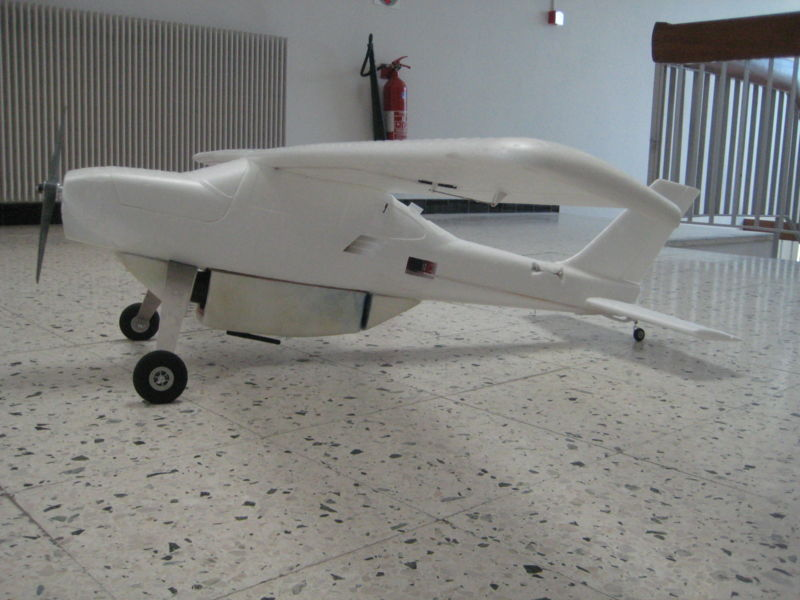
\includegraphics[width=10cm]{800px-Mentor1_2.jpg}
 % 800px-Mentor1_2.jpg: 800x600 pixel, 180dpi, 11.29x8.47 cm, bb=0 0 320 240
 \caption{Completed Mentor Aircraft with Payload}
 \label{fig:mentor}
\end{figure}

The major aircraft components are listed below:

\begin{itemize}
 \item Motor : AXI 2820 Gold Brushless DC
 \item Propellor : APC 11 x 7 
 \item Electronic Speed Controller : 80 Amp Brushless
 \item Batteries : 3 series elements Lithium Polymer
 \item RC Receiver : Multiplex 4 Channel modified to output PPM signal
 \item RC Transmitter : Multiplex Cockpit SX
 \item Autopilot: Tiny v1.1 with Ublox LEA-4H GPS receiver (Figure \ref{fig:tiny})
 \item Attitude Sensors : Infrared (6 orthogonal pixels paparazzi analog design see Figure \ref{fig:ir})
\end{itemize}

Power for the RC Servos is supplied by a stand-alone BEC (Battery Elimination Circuit) instead of using the power provided by the autopilot board. This is done to eliminate the possibility of power supply rail fluctuations due to the intermittent high current loads generated by the servos. The fluctuations can lead to the autopilot's processor rebooting in flight which can have dire consequences.

\begin{figure}[ht]
 \centering
 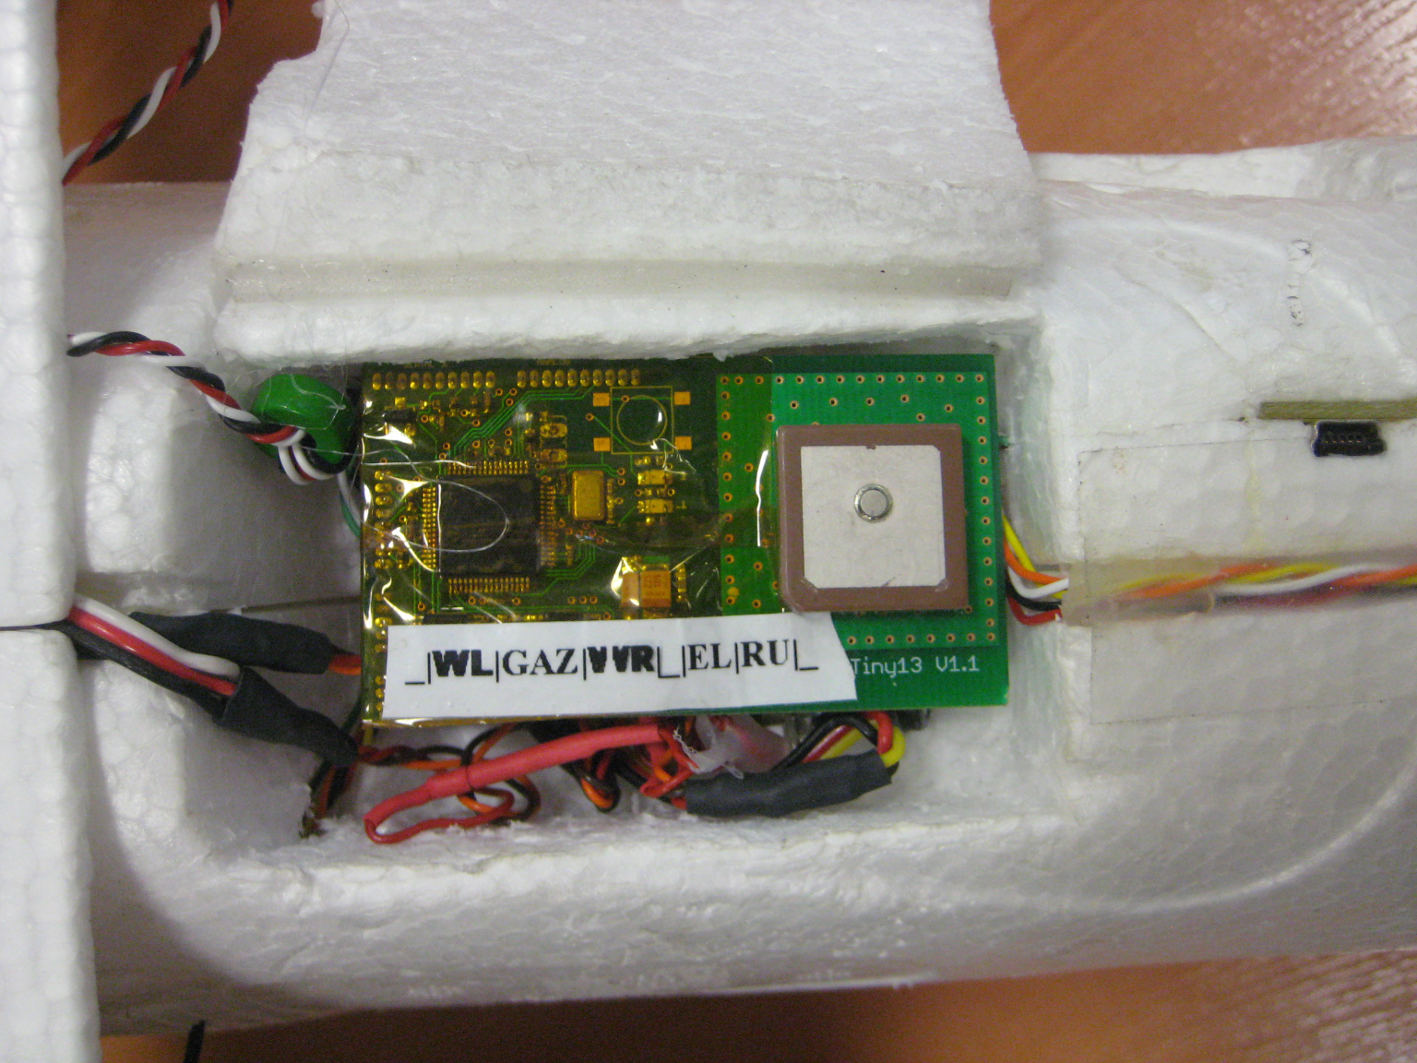
\includegraphics[width=10cm]{tiny_inside.png}
 % 800px-Mentor1_2.jpg: 800x600 pixel, 180dpi, 11.29x8.47 cm, bb=0 0 320 240
 \caption{Autopilot board installed in aircraft}
 \label{fig:tiny}
\end{figure}

\begin{figure}[ht]
  \centering
  \subfloat[IR Sensors as mounted in aircraft]{\label{fig:geo1}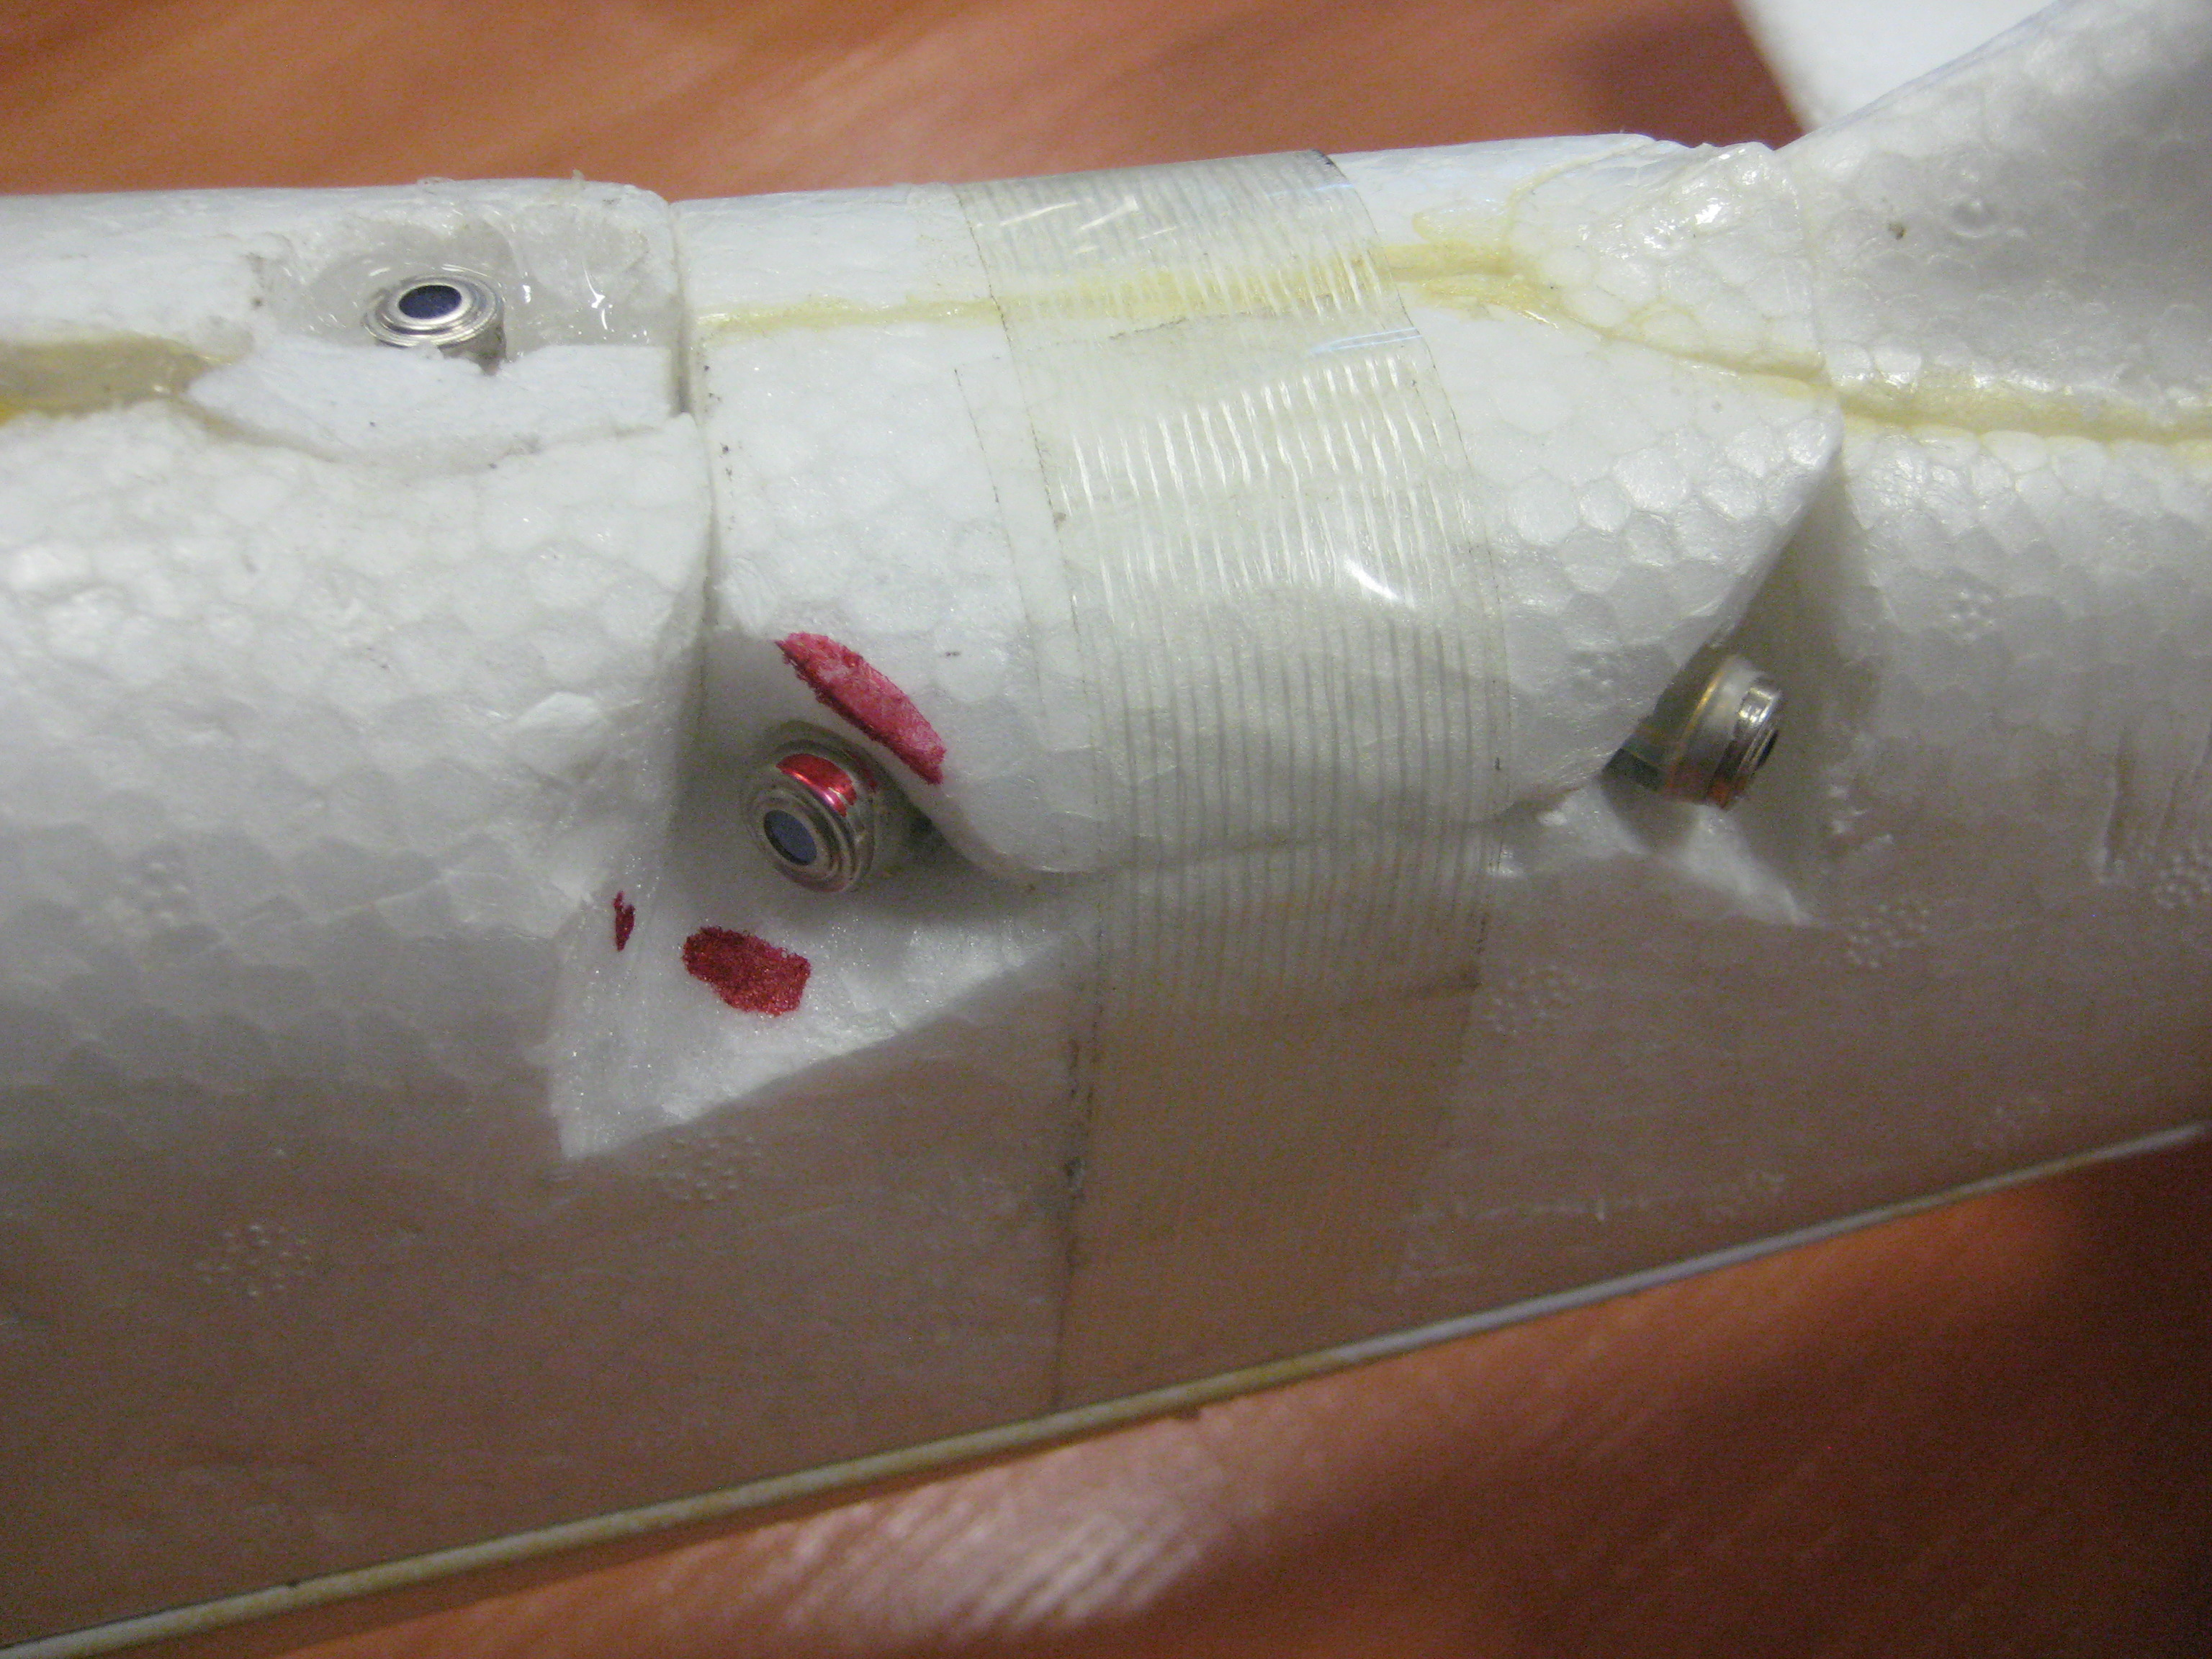
\includegraphics[width=90mm]{ir_closed.jpg}}                
  \subfloat[Board view of horizontal IR sensors]{\label{fig:geo2}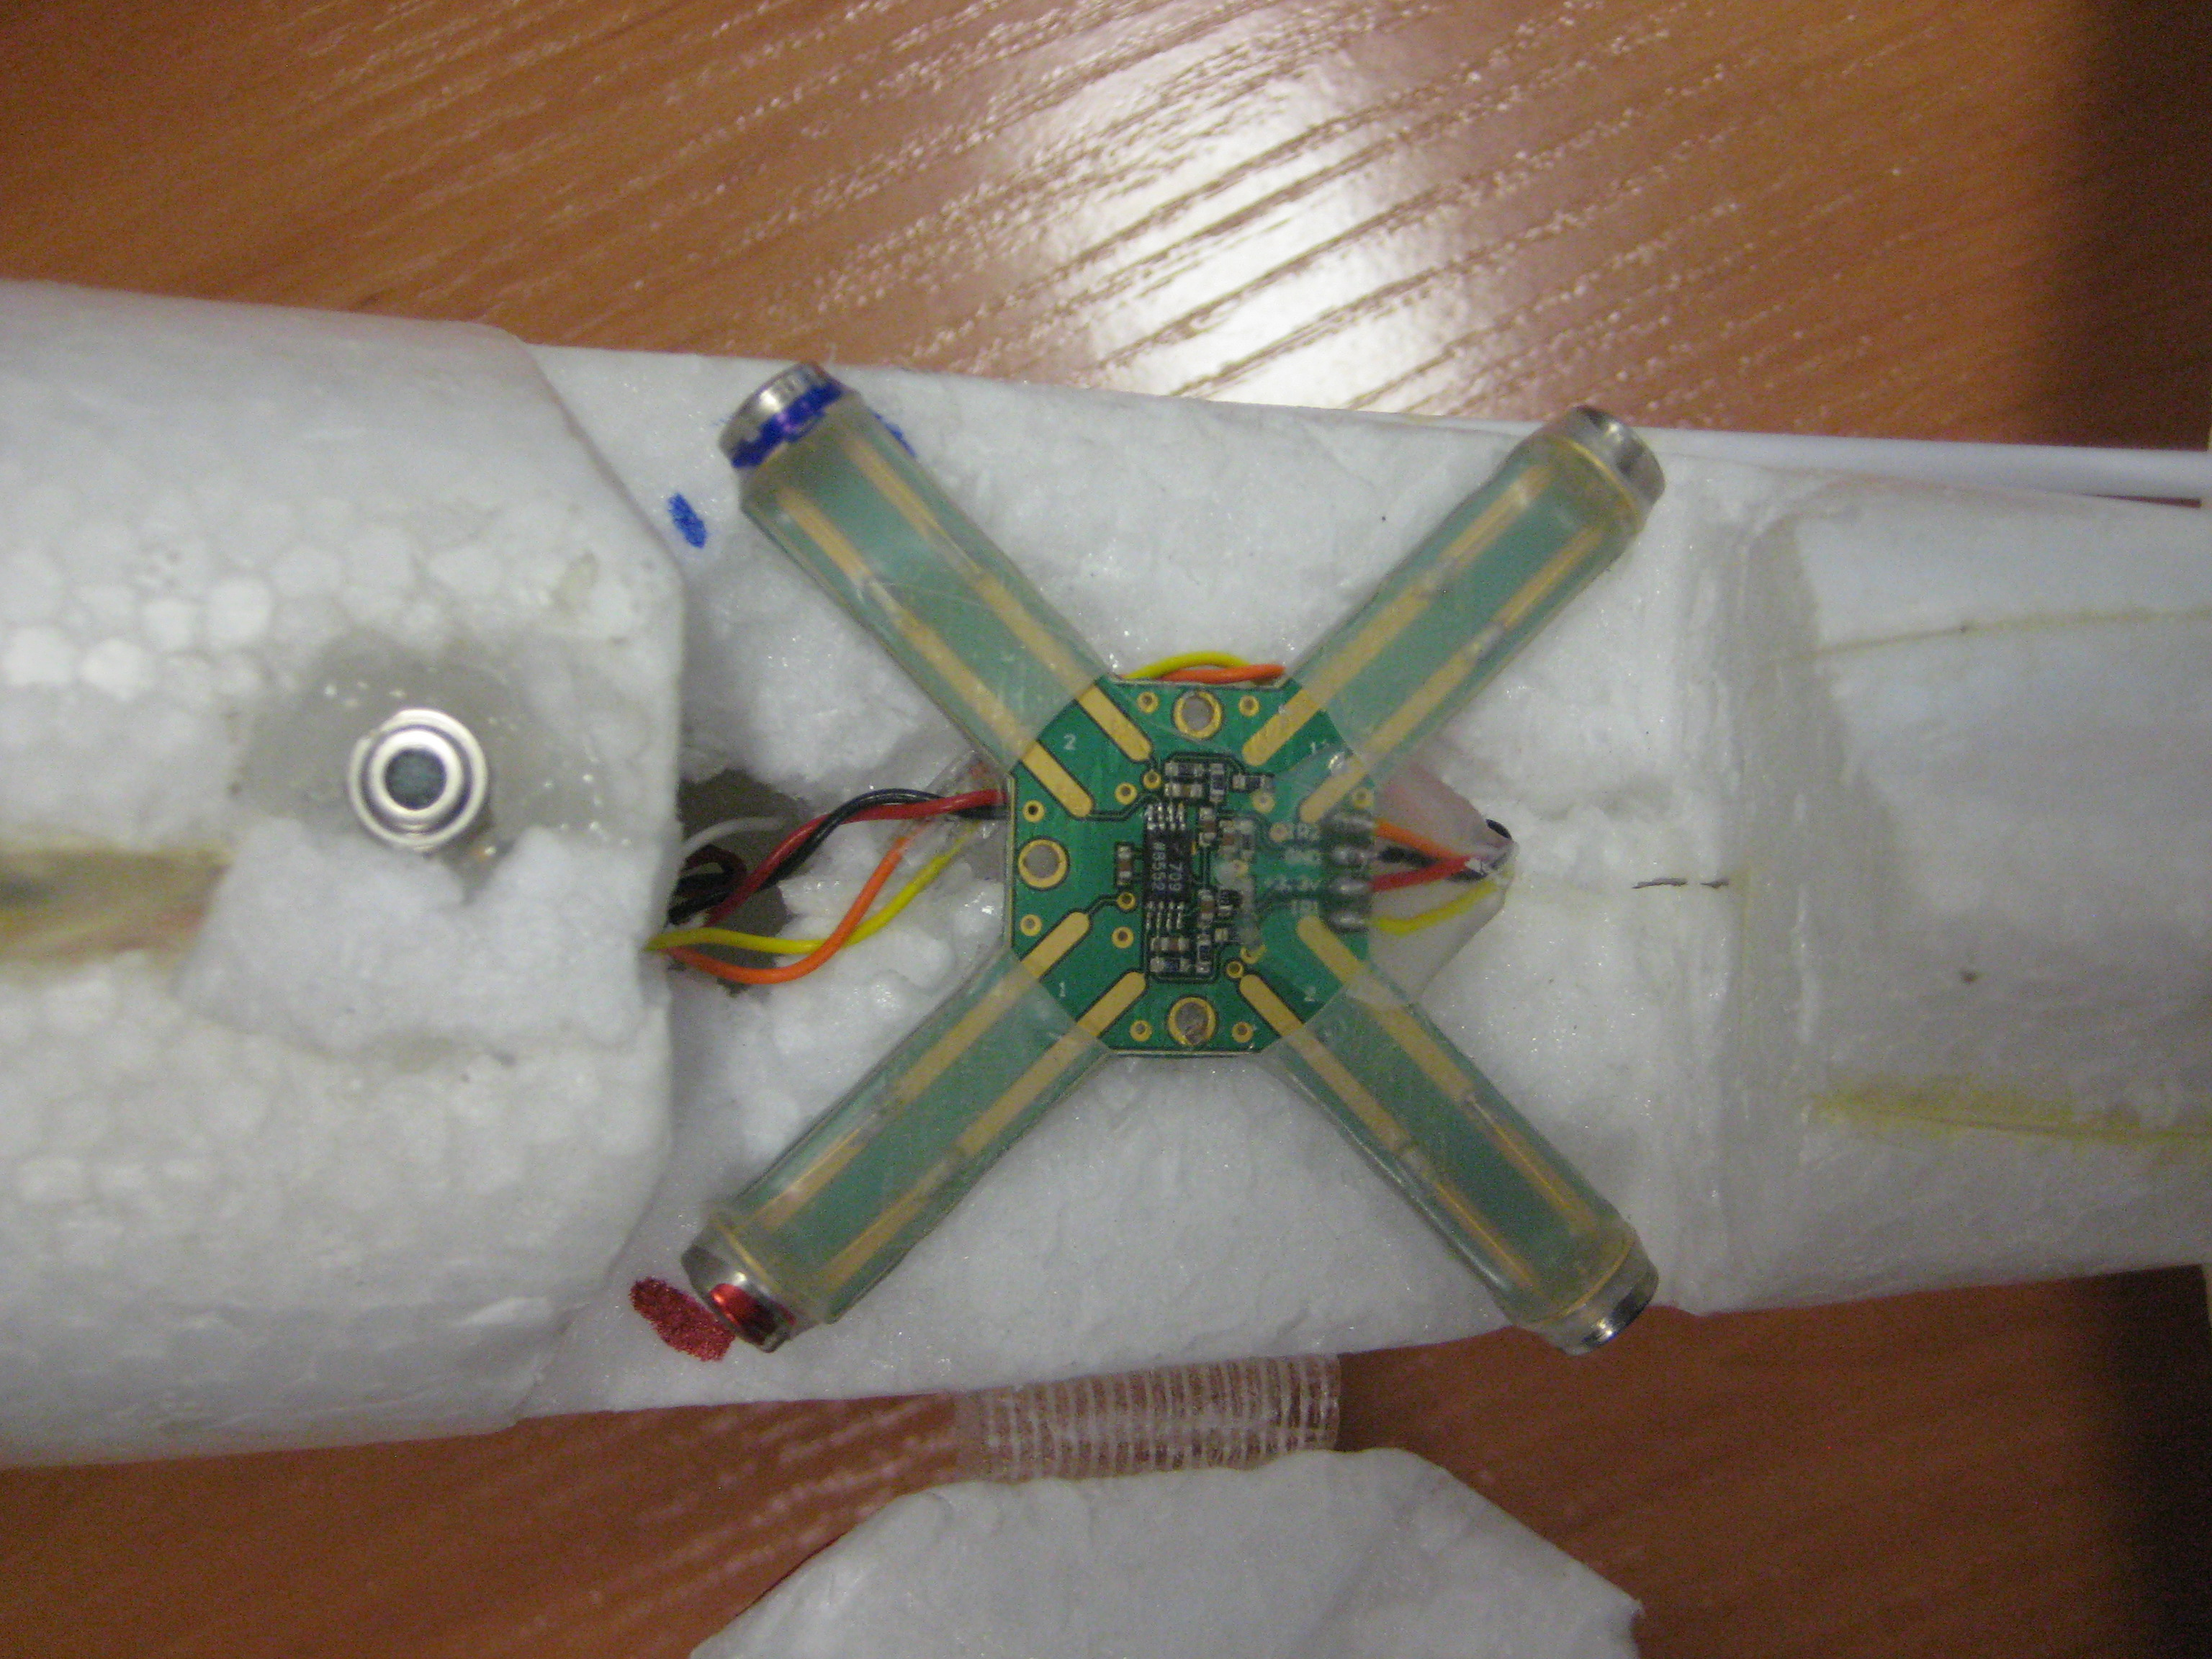
\includegraphics[width=90mm]{ir_open.jpg}}
  \caption{Autopilot Infrared Attitude Sensors}
  \label{fig:ir}
\end{figure}


\subsubsection{Airframe Parameters}

The airframe configuration file contains a number of parameters that are specific to the physical airframe and are used by autopilot. These characteristics such as minimum and maximum speed, control loop gains, servo ordering and positions, etc, are listed in an xml configuration file in Appendix A. Much of the initial flight testing is aimed at finding adequate gains to achieve tight control and navigation while maintaining stability in a variety of outdoor conditions. This is initially a tense and risky, itterative process. If the backup manual link with the safety pilot becomes unavailable when there's a control issue, the aircraft is sure to crash.

\subsection{Payload}

The payload pod is built using typical model construction techniques. As seen in Figure \ref{fig:payload}, a plywood frame houses the various components and a glass-fiber reinforced foam cover provides a streamlined shape and protects the pod contents in the event of a crash. I built it over the course of three weeks, paying attention to weight and strength. Cables are routed to minimize lengths, connectors are in positions that lend themselves to ease of use. The foam was cut with a hot-wire tool and sanded to an aerodynamic shape before covering with a thin layer of fiberglass and epoxy. 

I also build a test version of the payload for initial flights without the expensive hokuyo device (Figure \ref{fig:payload}). It is capable of carying a Canon SD750 digital camera in an integrated rotating servo mount. The construction permitted me to perfect my foam shaping and fiberglass covering techniques, and later, during field testing, the device proved useful for carrying incrementally larger weights as we gained confidence in the aircraft.

\begin{figure}[ht]
 \centering
 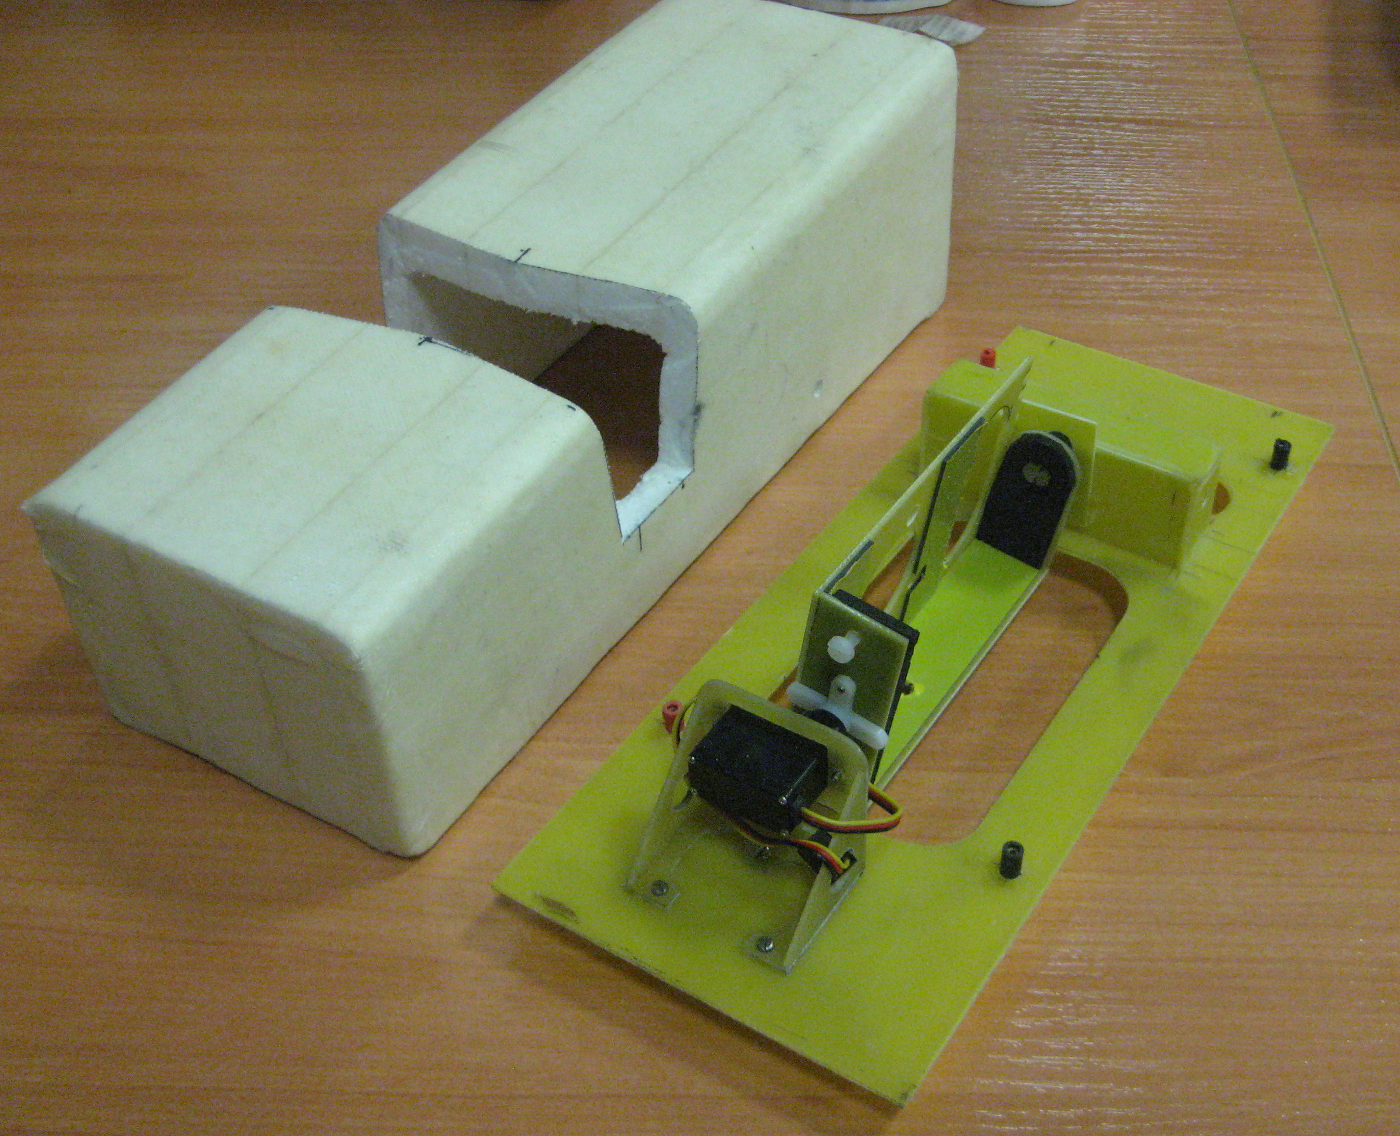
\includegraphics[width=12cm]{test_payload.png}
 \caption{Completed Test Payload Pod}
 \label{fig:test_payload}
\end{figure}

The payload is designed for quick insertion and removal from the aircraft, with a single magnetically-held carbon rod used to secure it to the craft. All of the payload electronics are self-contained and can be placed on a desk next to a work station without having to have the cumbersome aircraft present.

The payload weight is 650 grams which requires the Mentor to fly at higher than normal cruising speeds to generate the necessary lift. 

\begin{figure}[ht]
  \centering
  \subfloat[Payload]{\label{fig:weight1}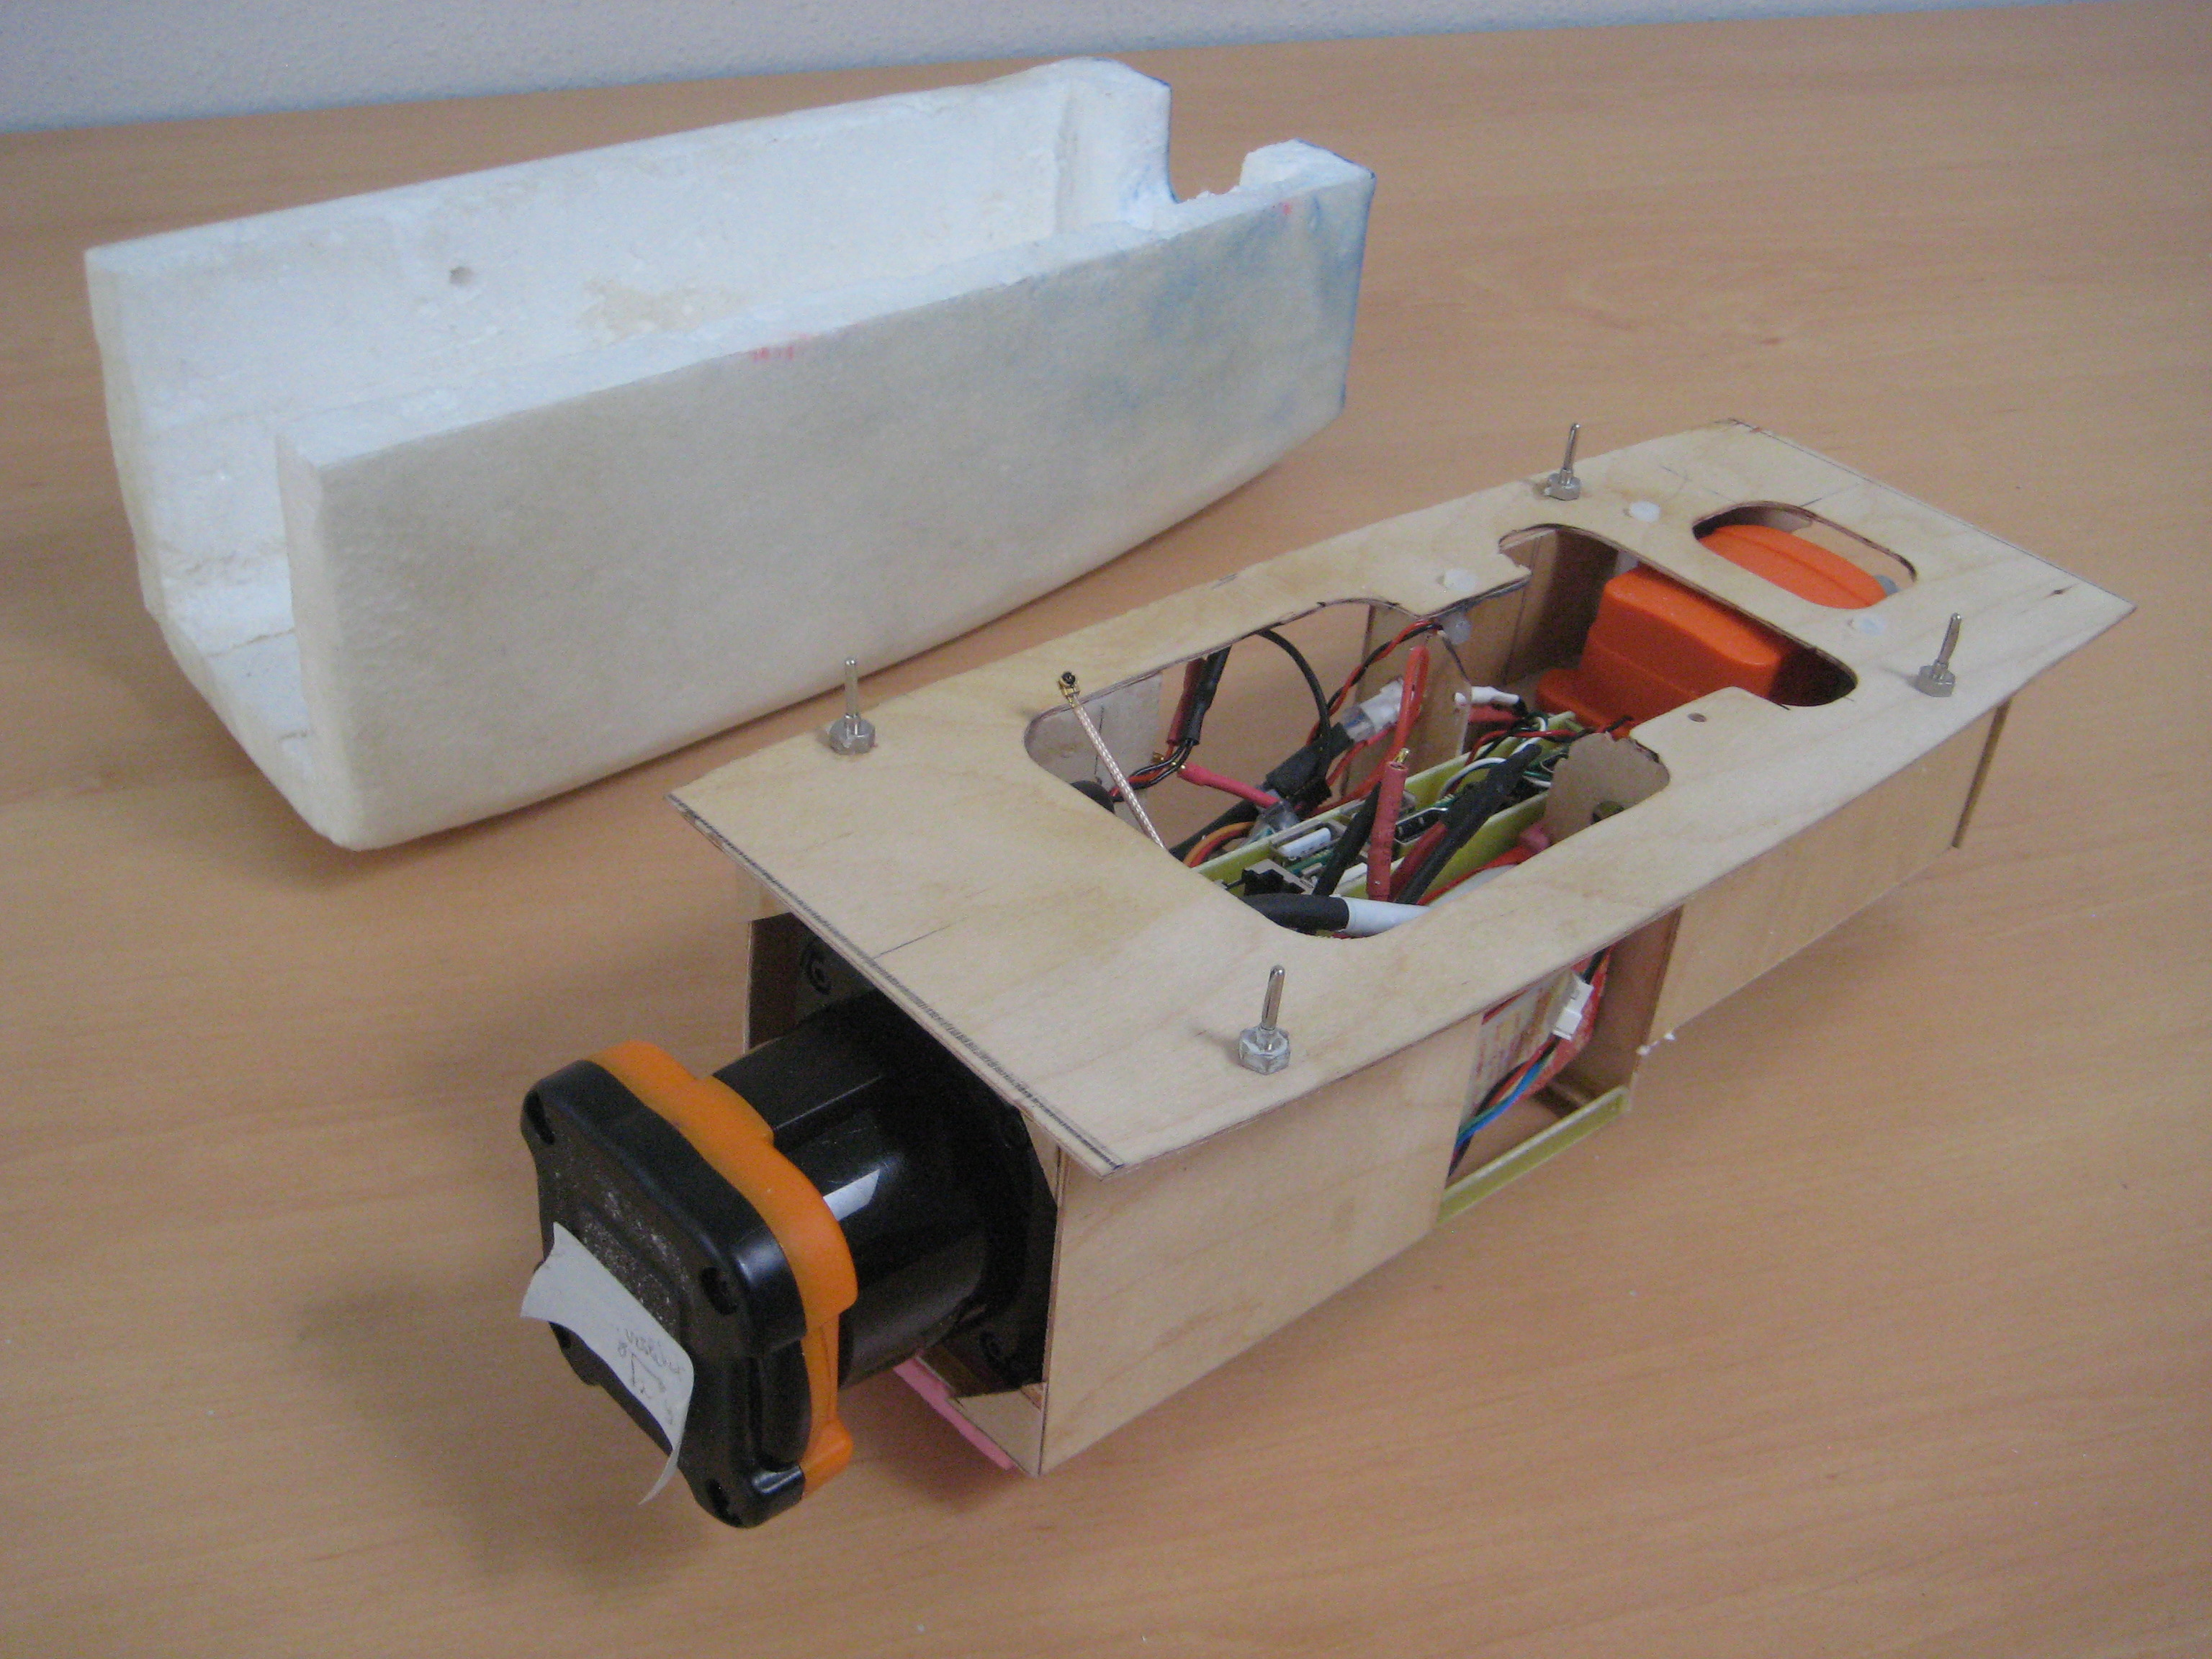
\includegraphics[width=90mm]{Mentor1_payload2.jpg}}                
  \subfloat[Overall]{\label{fig:weight2}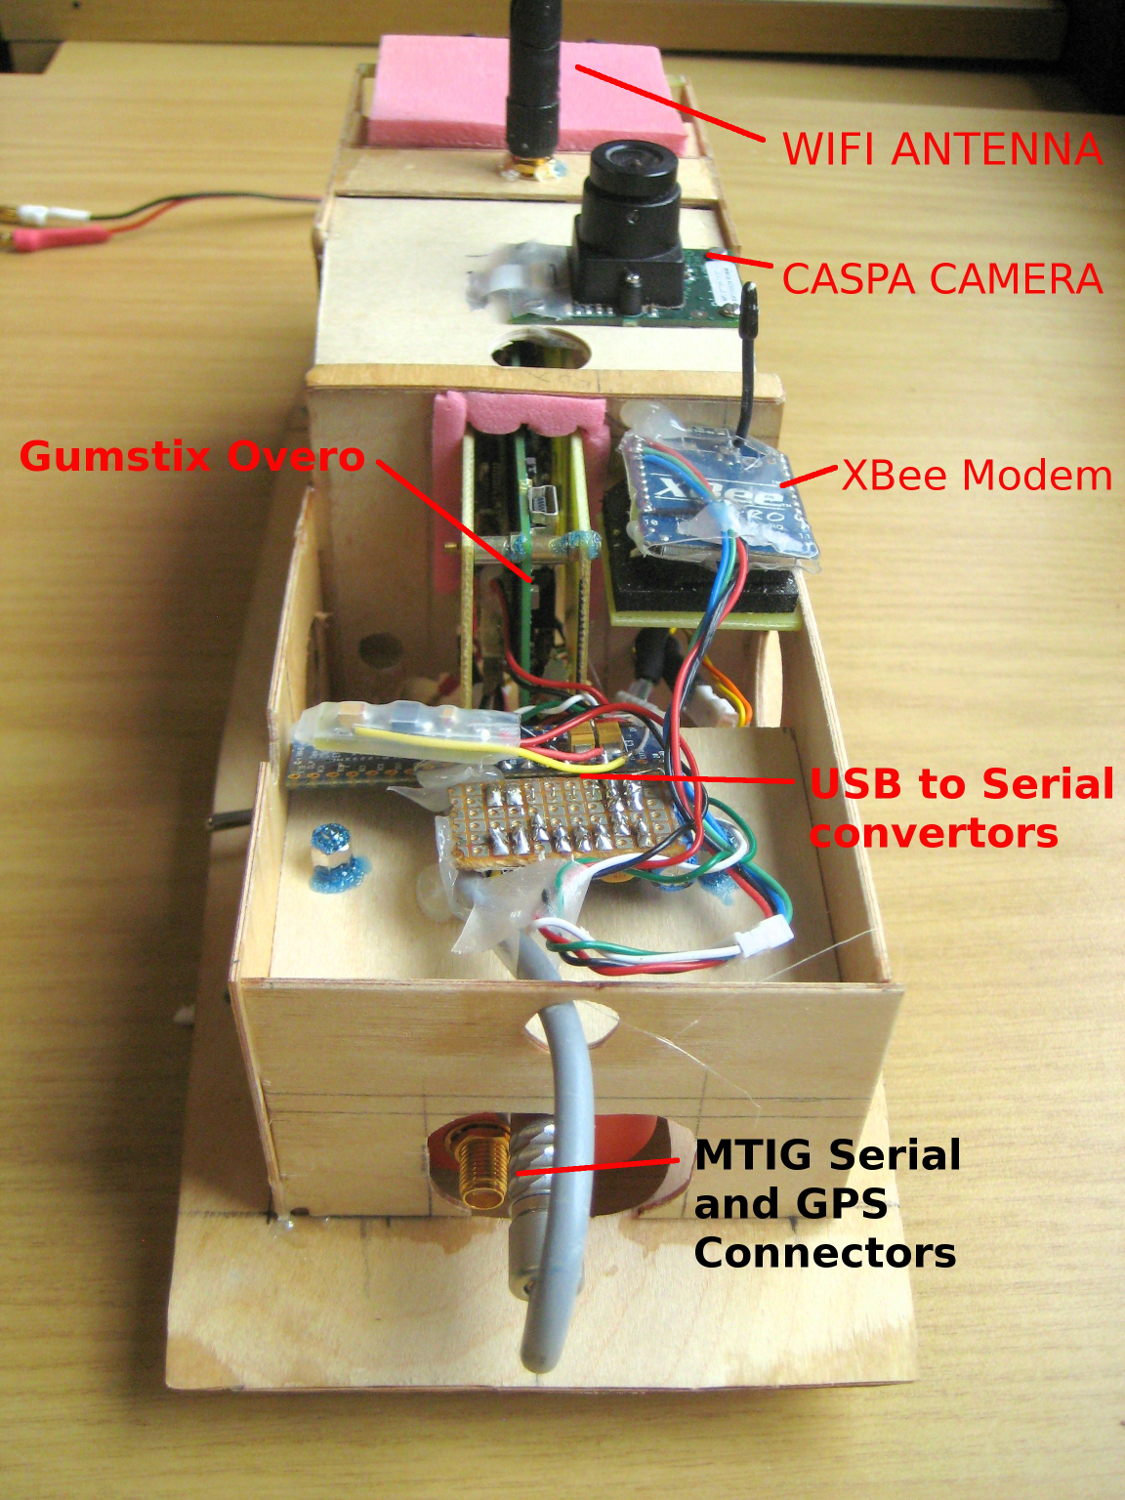
\includegraphics[width=90mm]{payload_internals.png}}
 \caption{Completed Payload Pod}
 \label{fig:payload}
\end{figure}

\subsubsection{Autopilot to Payload interface}

There is a three wire connection between the autopilot and the payload. It consists of a shared ground and two signals. The two signals are for the autopilot to monitor the payload battery, and for the payload to log the auopilot telemetry.

Lithium Polymer batteries require that a certain maximum discharge level (or a minimum voltage level) be respected to deter permanent damage. since the payload is powered by it's own independent LiPo battery, a connection to the autopilot was made to allow for monitoring the voltage level. To this end, a voltage divider I installed in the payload provides an output voltage compatible with the autopilot's ADC, and it is connected to a spare input channel on the autopilot board. The voltage level is sent to the ground station as an ADC\_GENERIC message and monitored directly by the ground control user by means of a paparazzi GCS papget (see Figure \ref{fig:papget}). The papget automatically does the conversion from raw ADC value to voltage reading. When the voltage level approaches the minimum allowed, the GCS operator can request the aircraft to land for battery replacement.

\begin{figure}[htb]
 \centering
 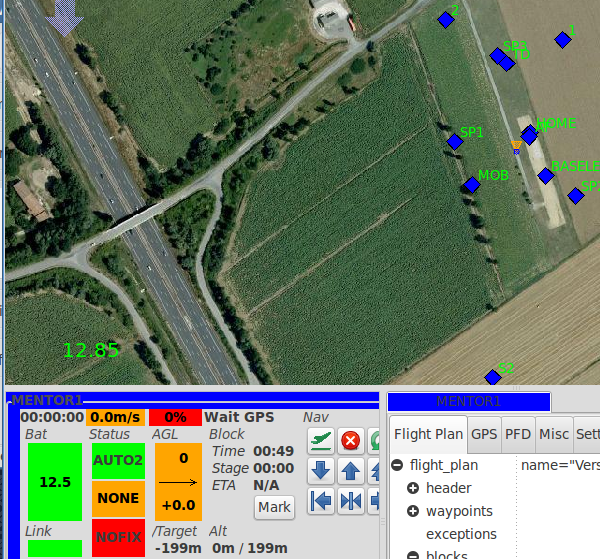
\includegraphics[width=12cm]{papget.png}
 % Mentor1_payload2.jpg: 3072x2304 pixel, 180dpi, 43.35x32.51 cm, bb=0 0 1229 922
 \caption{Paparazzi Ground Control Station with papget showing a payload battery voltage of 12.85V}
 \label{fig:papget}
\end{figure}

The second connection between the autopilot and the payload is that the autopilot's telemetry transmit output so that all raw traffic can be logged by the payload. The data is already logged on the paparazzi ground station (except for when the modems lose their connection), but this connection allows the payload to identify where in the cartography flight plan the aircraft currently is, which is useful for knowing when and how to capture and log most efficiently. 

Initially, we had a third connection in mind. To economize the payload battery we'd planned to switch the power provided to the Hokuyo in flight using outputs provided by the autopilot board. I designed and built a simple N-FET circuit designed to switch the payload battery's ground, but testing showed that cutting the ground connection of the Hokuyo scanner renders it permanently damaged. The issue is that the Hokuyo device has a second ground connection on it's USB connector. When the ground is cut on the power connector, current continues to flow into the device on the power supply rail and flows out of the USB ground which is not capable of handling the current. The device had to sent to the manufacturer in Japan for repairs which took over two months.

\subsubsection{Block Diagram}

The payload electronics hardware is connected as per the block diagram in Figure \ref{fig:hwdiagram}.

\begin{figure}[htb]
 \centering
 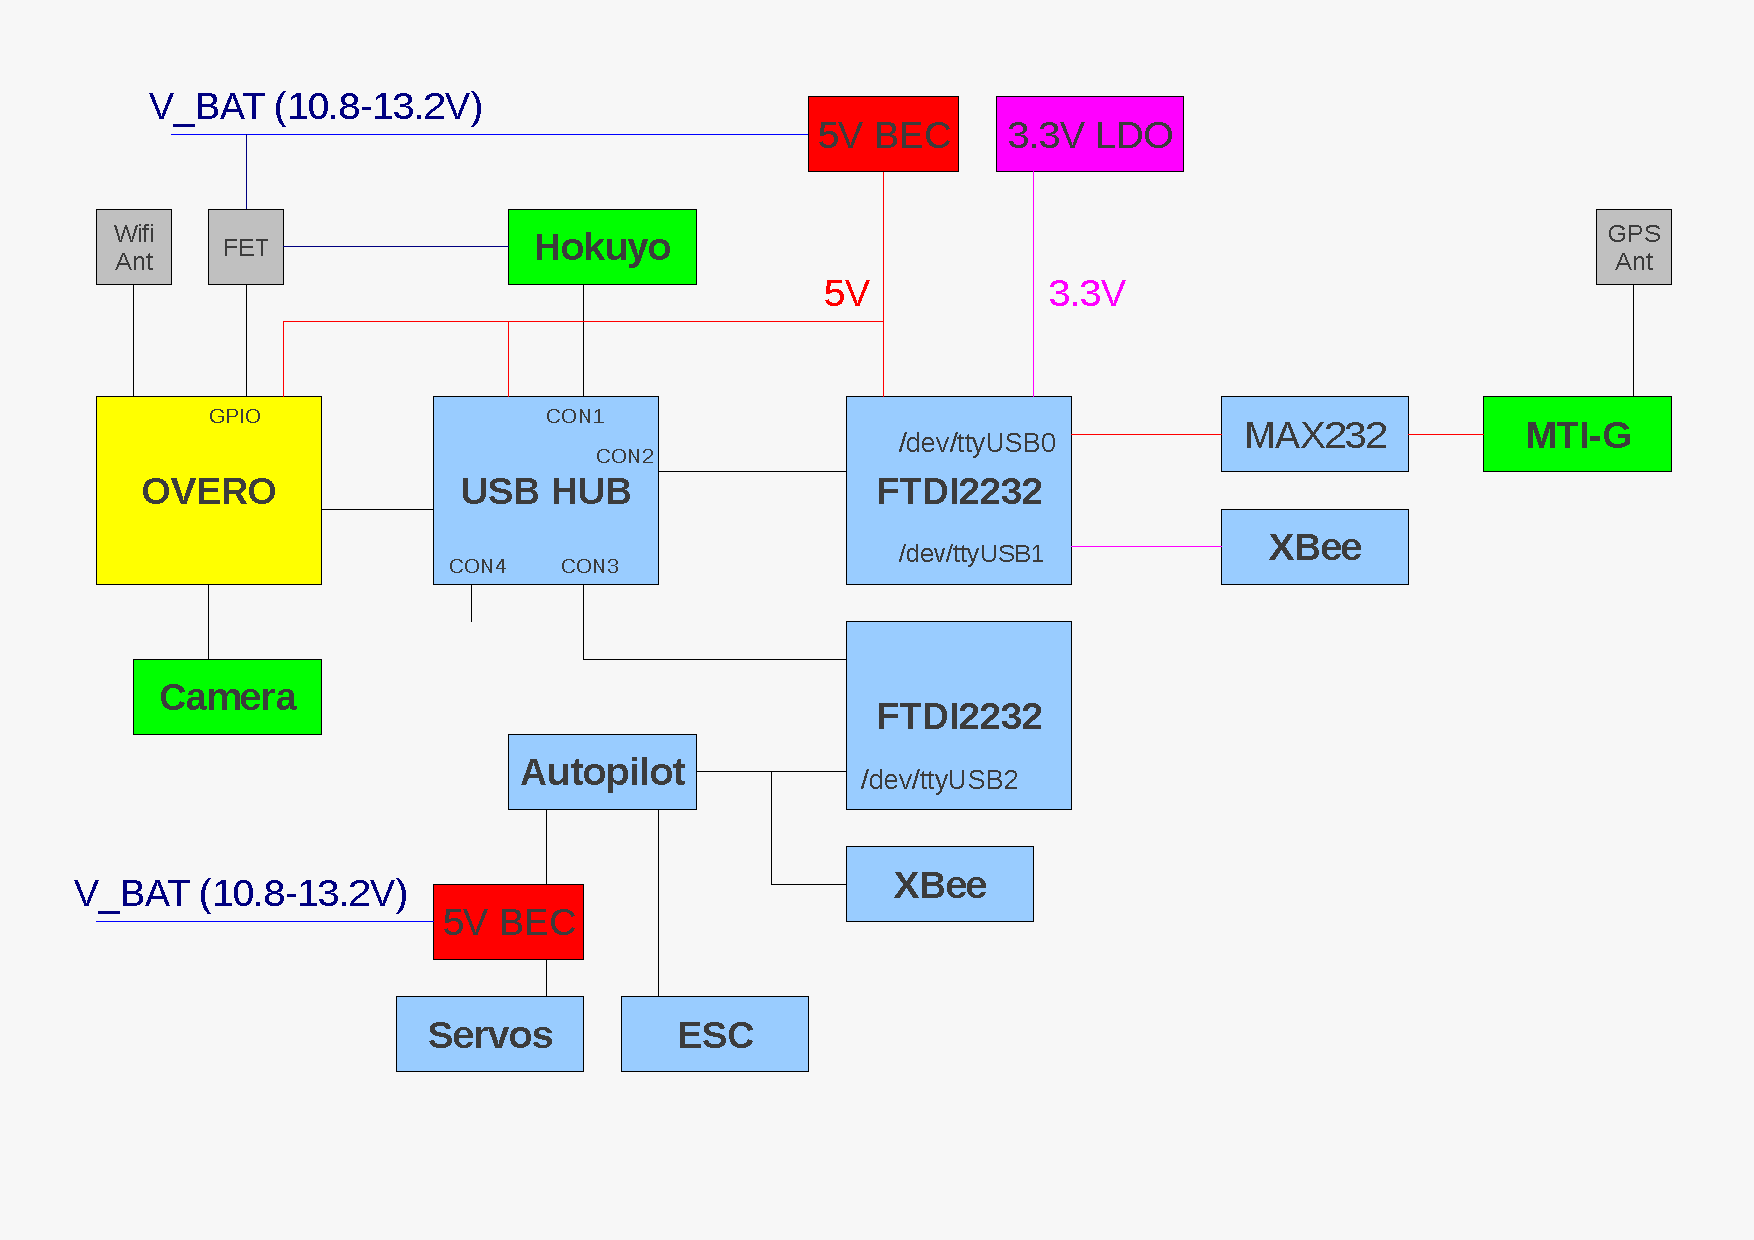
\includegraphics[width=12cm]{Payload_hardware_block_diagram}
 % Payload_hw_block_diagram.png: 0x0 pixel, 300dpi, 0.00x0.00 cm, bb=
 \caption{Payload Hardware Block Diagram}
 \label{fig:hwdiagram}
\end{figure}

\subsubsection{Weights}

The weight of the individual components are listed in Figure \ref{fig:weight1} and \ref{fig:weight2}.

\begin{figure}[htb]
  \centering
  \subfloat[Payload]{\label{fig:weight1}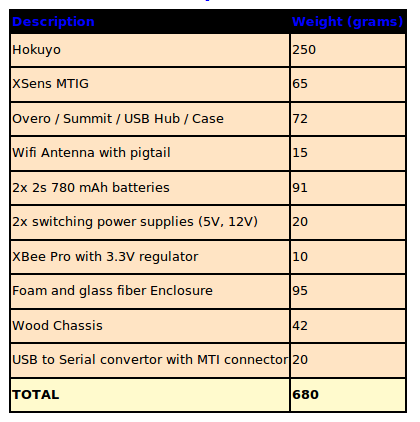
\includegraphics[width=70mm]{weights.png}}                
  \subfloat[Overall]{\label{fig:weight2}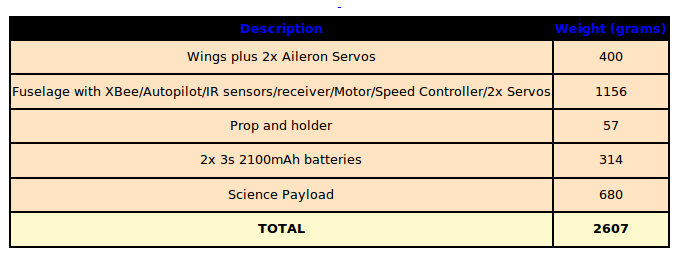
\includegraphics[width=105mm]{weights_overall.png}}
  \caption{Aircraft Weights}
  \label{fig:weights}
\end{figure} 

\subsection{Cartography Flight Plan}

To request the UAV to fly in parallel tracks above a region of interest, we created a custom flight plan and navigation function and merged it into the paparazzi source code base. The function allows a region of interest to be defined either before or in flight by the GCS operator by defining three waypoints. These waypoints define a area for which the autopilot calculates two sets of overlapping parallel tracks, each set perpendicular to the other. The aircraft then flies along these tracks as best as possible given wind conditions and other challenges. Figure \ref{fig:gridcarto} shows the cartography function in action. In the figure, the aircraft can be seen near the center of the image traversing the current ground track highlighted in green. The aircraft track in blue shows the UAVs trajectory since the start of the pattern. The region of interest is defined by the waypoints named S1, S2, S3, and S4, and the tracks within the region are all straight lines.

The current cartography function assumes a constant altitude during the entire pattern. Due to the limited laser scanner range of 10-15 meters, this method would only work in relatively flat terrains and without large obstacles such as trees or buildings.

\begin{figure}[ht]
 \centering
 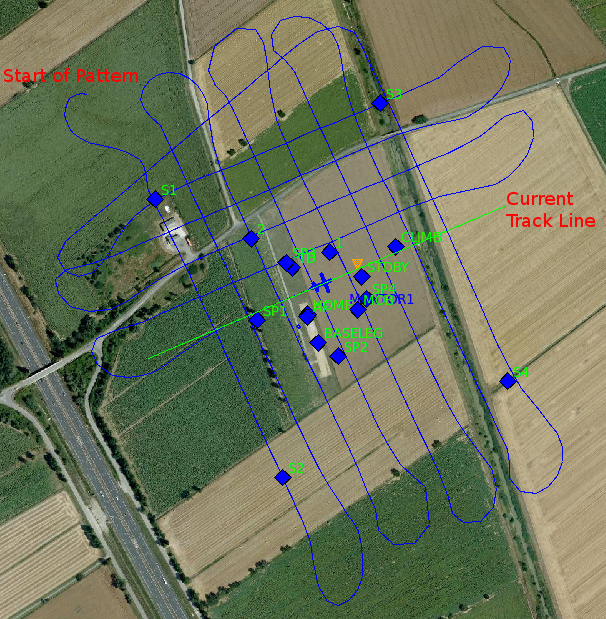
\includegraphics[width=10cm]{pprz_cartography.png}
 \caption{Grid Cartography Flight Plan}
 \label{fig:gridcarto}
\end{figure}

\chapter{Results}

This chapter details our flight testing along and describes our most significant discoveries and challenges.

\section{Flight Tests}
\label{flight_tests}

Flight testing was performed at a small model airfield on the southern outskirts of Toulouse (Deyme). The site is situation in the midst of wheat fields. There is a small covered work area on site and a row of medium-sized trees. Less than 200 meters away is an irrigation ditch, a road bridge, and some small warehouse buildings. A satellite view of the terrain is visible in Figure \ref{fig:gridcarto}, and a picture of the drone in flight with the test payload in Figure \ref{fig:pay1} and with our real payload in Figure \ref{fig:pay2}.

\begin{figure}[ht]
  \centering
   \subfloat[With test payload]{\label{fig:pay1}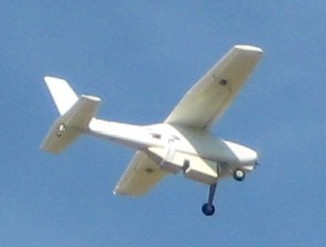
\includegraphics[width=80mm]{mentor_in_flight.JPG}}                
   \subfloat[With real payload]{\label{fig:pay2}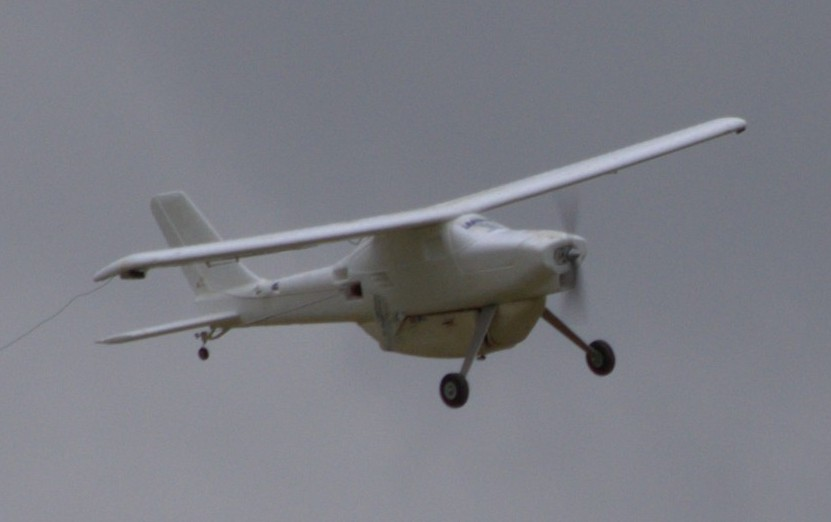
\includegraphics[width=95mm]{mentor_low.jpg}}
  \caption{Mentor and Payload in Flight}
 \label{fig:mentor_flying}
\end{figure}


The flight tests were done over many weeks, each time with progressively more equipment integrated on board. Flight tests typically involved loading up the LAAS van around 2 or 3 pm, a half an hour travel to the field, a few hours on the field and a return around 7 to 8 pm. Logs of the main flights are stored in the project repository (\cite{laserhawkgit}) and include the following :

\begin{itemize}
 \item Feb 17 - manual flights at Muret (no autopilot)
 \item Apr 20 - with autopilot and payload, ground tests at ENAC
 \item May 11 - 2 flights at Deyme
 \item May 17 - 6 flights at Deyme
 \item May 19 - 3 flights at Deyme
 \item May 23 - 2 flights at Deyme
 \item May 26 - 4 flights at Deyme
\end{itemize}

The first flights without autopilot were to prove the airframe could handle takeoffs, landings, and was stable under manual control and resulted in a number of elements requiring fine tuning. The landing wheels had to be adjusted and the propellor replaced with a large one to provide more thrust during takeoff. Lab testing showed the larger propellor increased the motor's maximum current draw beyond the 40 A rating of our current motor controller so I replaced it with an 80 A controller. 

In the following flight tests, we began to test autonomous flight. ''Auto1'' mode, where the autopilot regulates the aircraft attitude based on angle setpoints provided by the RC transmitter, was tested and the process of adjusting gains could begin. We struggled with the autopilot providing erratic attitude readings. The vertical readings were fluctuating wildly, and the aircraft randomly would estimate itself to be on it's back. When the vertical IR sensor was removed, the source of the problem became apparent. The op amp circuit was poorly soldered and intermittent connections on the IC pins were visible. Replacing the vertical IR sensor board with a newly built one resolved our issue and test flights could resume.

We continued flights while tuning parameters to achieve ``Auto2'' mode where the aircraft navigated on it's own while following the flight plan. Further flights proved the weight carrying capacity of the platform as we increasingly added dead weight until we reached the target required to carry our real payload. At the maximum weight, the capacity to climb reduced significantly, runway distance increased, but these remained reasonable. Cruise speed of 15 m/s required only half-throttle and autonomy using our 5000 mAh batteries permitted 10 to 12 minute flights so the aircraft in general looked like it would be a success.

Since we had many days of rain and high winds in May and June, we had the additional challenge of working around the weather. Some days we would arrive at the field to find the wind too violent to allow us to fly. Other times, we would forget a crucial piece of equipment (our payload's SD card that contains all of our software), or a piece of equipment would stop functioning completely (most notably, a servo). Other chalenges included coordinating with the hobyist onsite who were actively taking off and landing regularly. Their loud gas engine planes and helicopters often made communication between pilot and ground controller impossible.

Our biggest struggle was the fact that our R/C link, which is used to manually fly the plane if there is an issue with the autopilot, often had a very limited range. Ground tests showed the link did not extend to the edge of the flying field. This is a dangerous situation that makes safe flight impossible and makes landing particularly challenging. As the aircraft approaches the runway for landing, it's proximity to the ground further reduces the RF range and a loss of control, even for less than a second, can lead to a crash. In order to isolate the R/C receiver from the RF environment, I enclosed it in a small grounded iron cage, and did the same for the onboard BECs whose switching power regulators are notorious for EMI generation. Field testing showed the improvements were modest at best. On a hunch, we built a number of different length cable extensions to allow placing the receiver away from the fuselage. Our tests showed that the best link quality was with the receiver placed at the tip of the wing as seen in Figure \ref{fig:pay2} with a cable length of nearly one meter. Link quality continues to this day as less than ideal, being around 200 meters near the ground, but is enough to permit continued tests flights.

Luckily, our most significant loss to date was the loss of our cockpit with integrated GPS antenna. It came off the aircraft during flight above wheat fields. It occured when the autopilot was being switched into manual mode and the aircraft was at low altitude. The pilot (my mentor) could not follow the foam piece for long as he had to concentrate on landing, and I was monitoring the ground station and never saw the piece fall off. We spent a few late hours looking for it, to no success. We had enough spare parts back at the lab to where I was able to make another the next day.

\begin{figure}[ht]
  \centering
  \subfloat[Ground Control in back of truck]{\label{fig:weight1}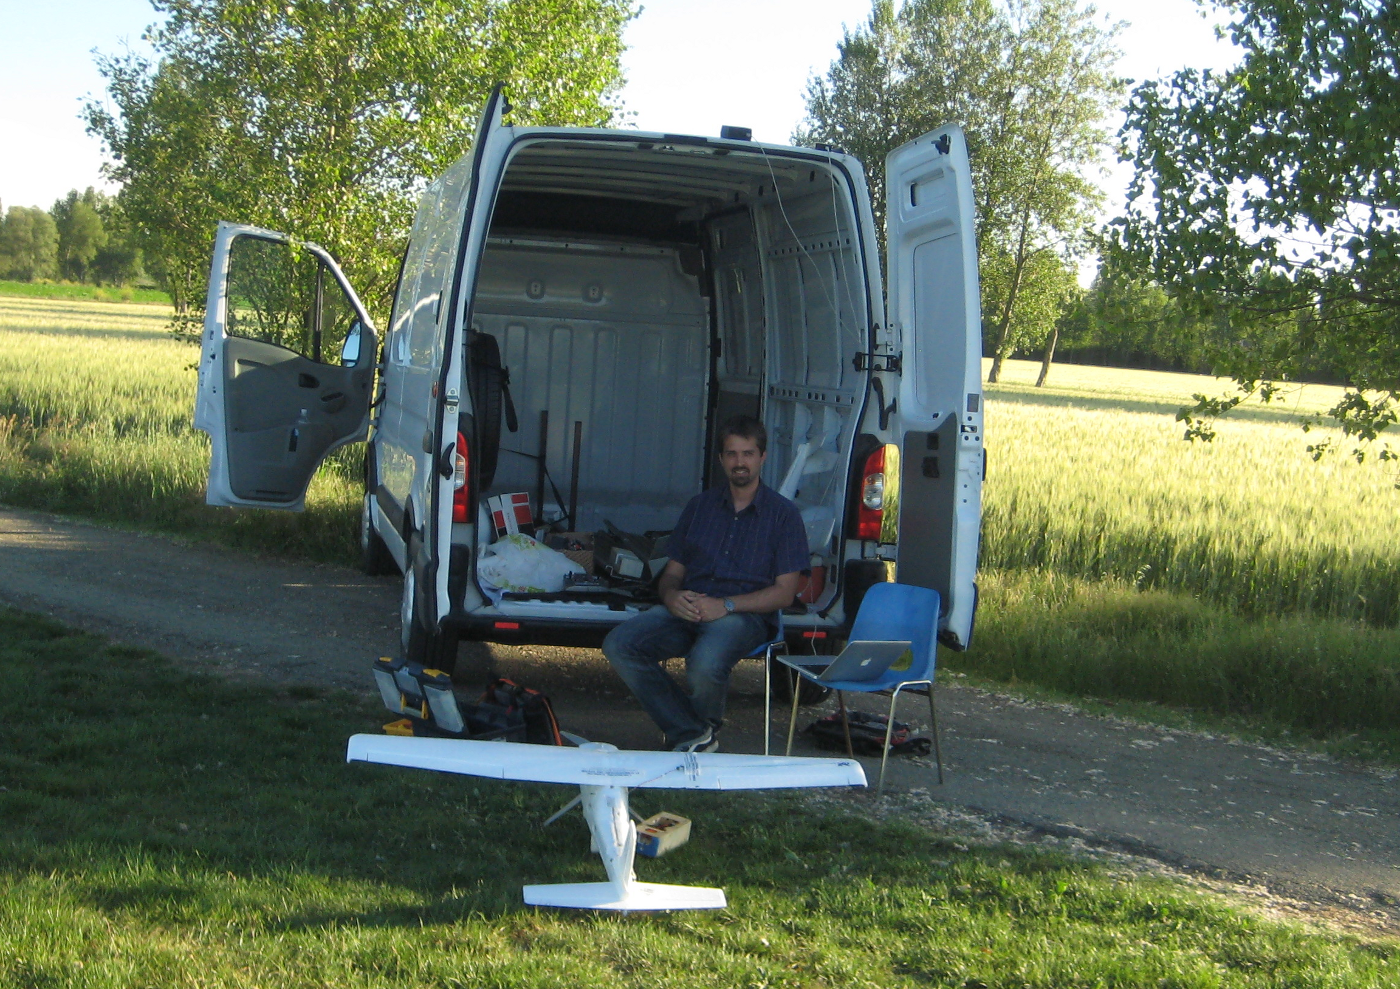
\includegraphics[width=83mm]{paul_at_deyme.png}}                
  \subfloat[Deyme Runway]{\label{fig:weight2}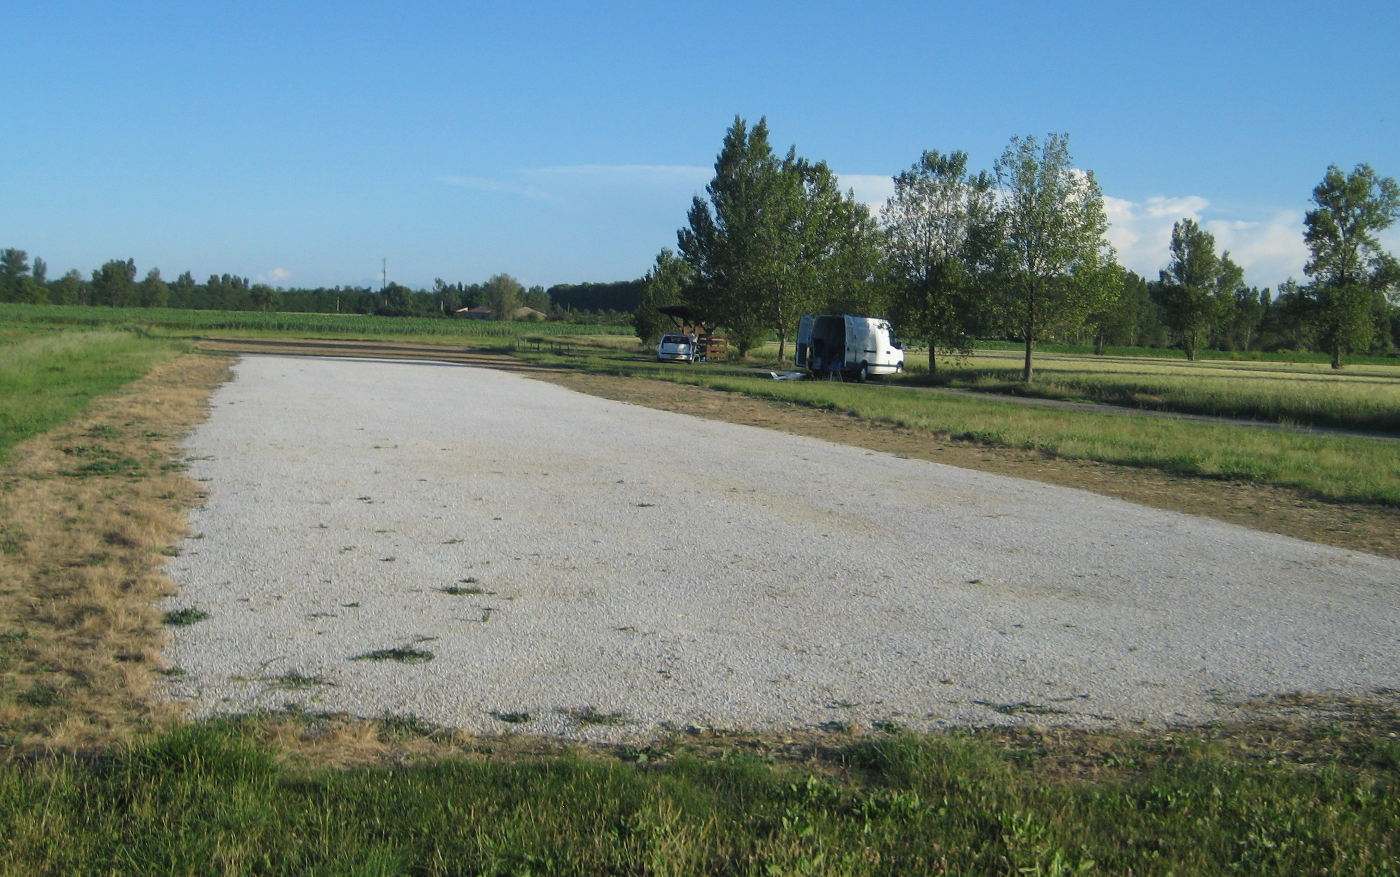
\includegraphics[width=95mm]{deyme_runway.png}}
  \caption{Deyme Field}
  \label{fig:field_shots}
\end{figure} 

\subsection{Multi-Robot Cooperation}

Since the ultimate cartographic goal of the project is to assist ground robots displace themselves in an unknown environment, the whole system must be considered. Defining what data will be treated and where is important as airborne processing power is severly limited but so is the bandwidth of the communication links. For air to ground robot communication, we included in our payload a serial modem identical to the one used by the autopilot telemetry link but on a different 2.4GHz channel. Using an access point on site, the wifi link proved to be very reliable in our field testing. So within a km or so our communication can comfortably proceed on the order of 10Mbps, while beyond that we're limited to 56kbps or potentially 115.2kbps. In the case of wifi, transfering raw data for the ground robot to process is conceivable (althoug with a low camera acquisition rate), while in the later case, the data will need to be either processed or reduced to its bare essentials and compressed. 

Beyond these computational and communication details lies the whole problem of how to best integrate this UAV-acquired data into the ground robot model of the environment. This is out of the scope of the current report, but I've begun to look into the way the environment is modeled on LAAS robots and how probabilistic traversability maps are used to compute near-term and long-term trajectories for displacement of a UGV. Some details are available in \cite{redouane_paper}.

\section{Hokuyo Lidar Performance}
\label{hokuyo_perf}

\subsection{Limited Lidar Range}

Using test flight data, the ability of the lidar sensor to detect the distance to the ground surface was determined by plotting the number of echoes detected for varying aircraft altitudes. The resulting plot as seen in Figure \ref{fig:lidar_perf} shows the inability to detect all echoes starts at an altitude of 9 meters. 

\begin{figure}[ht]
 \centering
 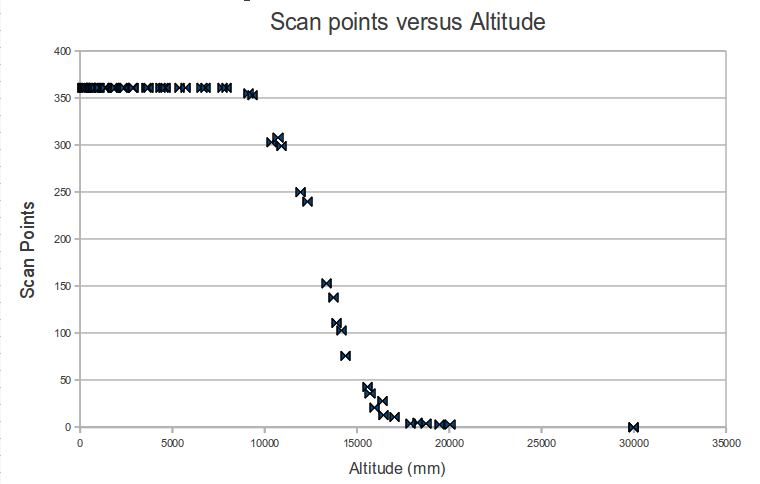
\includegraphics[width=12cm]{scanpt_v_alt.png}
 \caption{Lidar Range Performance in Flight}
 \label{fig:lidar_perf}
\end{figure}

The number of echoes received in the 90 degree scan region should be 360 as the resolution is four points per degree. Assuming the aircraft is horizontal, the 360 points represent the terrain profile along the scan path whose length is 2x the altitude. So, at 10 meters altitude we are imaging 20 meter swaths (Figure \ref{fig:lidar_scan1}). At 15 meters altitude, due to the sensor range limitations, the swaths imaged are much narrower than expected, in the 6 to 9 meter range (Figure \ref{fig:lidar_scan2}). Such narrow swaths require the flight plan to increase the number of back and forth flight trajectories over a given region of interest to decrease the spacing between them. This increases the time needed to cover a region, and for a given autonomy of 10 minutes reduces the size of the areas that can be scanned.

The laser scan test was done in a favorably cloudy day as can be seen in Figure \ref{fig:pay2}. Performance on a clear day is presumed to be inferior and will be quantified in future tests.

\begin{figure}[ht]
 \centering
 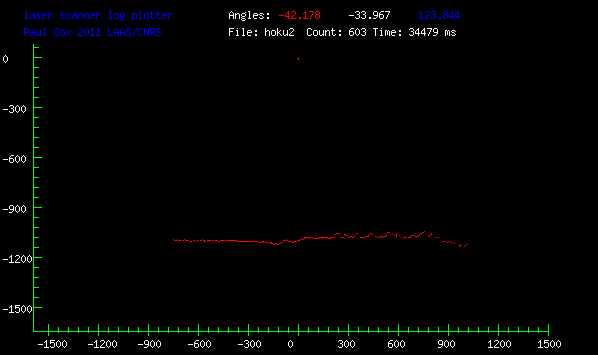
\includegraphics[width=12cm]{scan603.png}
 \caption{Typical Lidar Scan at apx 10 m altitude}
 \label{fig:lidar_scan1}
\end{figure}

\begin{figure}[ht]
 \centering
 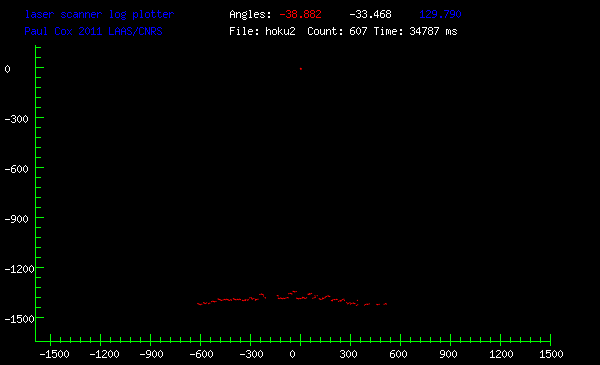
\includegraphics[width=12cm]{scan607.png}
 \caption{Typical Lidar Scan at apx 15 m altitude}
 \label{fig:lidar_scan2}
\end{figure}

\subsection{Lidar Driver Limitations}

Transferring the 1081 scan points at 40 scans per second requires considerable CPU time by the scanner driver. If the system is busy with other tasks such as writing to logs, or the compression and transfer of data to the ground station, the processor can be preempted and scans are lost as there is no scan buffering. Also, the scan intensity data is available but it's use leads to a 3-fold decrease in the effective scan rate so we opted not to read it. Finally, a multi-echo feature in the driver appears to only be possible with a different Hokuyo product.

\section{MTIG}

Initial testing showed an issue with the buffering of MTIG data. Much of the data was in clumps and the GPS position did not closely follow what was logged by the autopilot. Figure \ref{fig:track_comp} shows a comparison of GPS track recorded with the autopilot and the payload.

After some time working with the device driver library we discovered it was a problem in how the software was implemented. The issue caused much of the data to be lost, the timestamps to not reflect correct acquisition time, and high CPU utilization. 

\begin{figure}[ht]
  \centering
  \subfloat[Autopilot GPS]{\label{fig:ap_gps}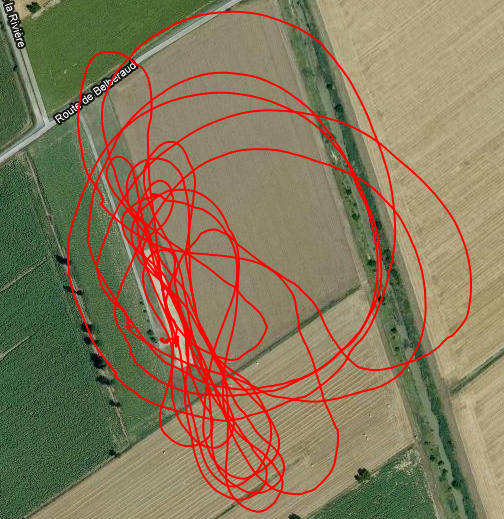
\includegraphics[width=70mm]{11_05_26__17_08_52_pprz_gmap.png}}                
  \subfloat[Payload GPS]{\label{fig:payload_gps}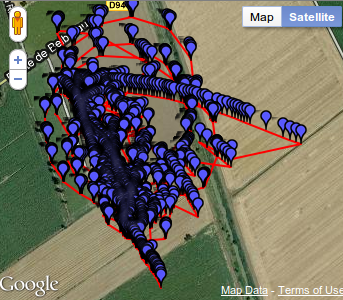
\includegraphics[width=82mm]{hoku2_flight_payload_gps.png}}
  \caption{GPS Tracks}
  \label{fig:track_comp}
\end{figure} 

\section{Caspa PX}

A camera device driver was available from the manufacturer in the form of a Linux kernel bitbake recipe, and it compiled and detected the camera. The camera flat-flex connector proved to be extremely fragile and a constant nuissance, but indoor camera tests showed we could capture images and videos and record them to disk. 

Initial image snapshots from the aircraft showed extreme over exposure. We attempted manual and automatic exposure modes, with no improvements. After trying many other device driver options, we determined that the HDR (High Dynamic Range) mode, which worked well in an indoors environment, caused this over exposure when we were outside. The camera's focus needs to be manually adjusted and the ideal setting during flight has yet to be determined, but sample images are presented in Figure \ref{fig:caspa_sample}.

\begin{figure}[ht]
  \centering
  \subfloat[My advisor as seen from UAV camera]{\label{fig:caspa_im1}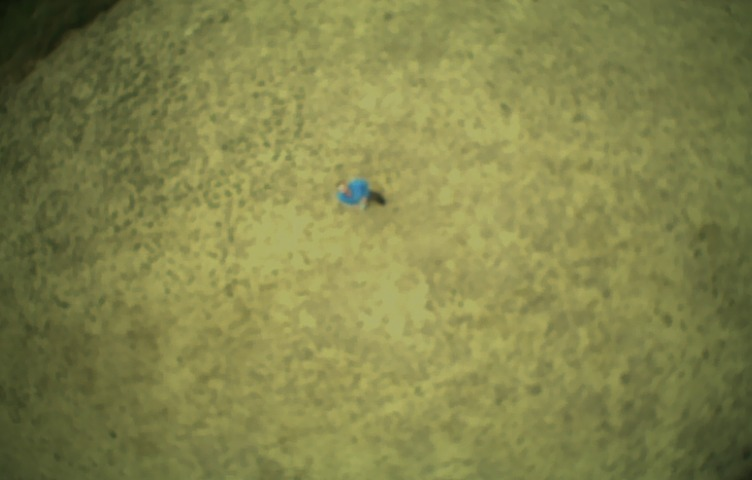
\includegraphics[width=80mm]{im13.jpg}}                
  \subfloat[A crop field]{\label{fig:caspa_im2}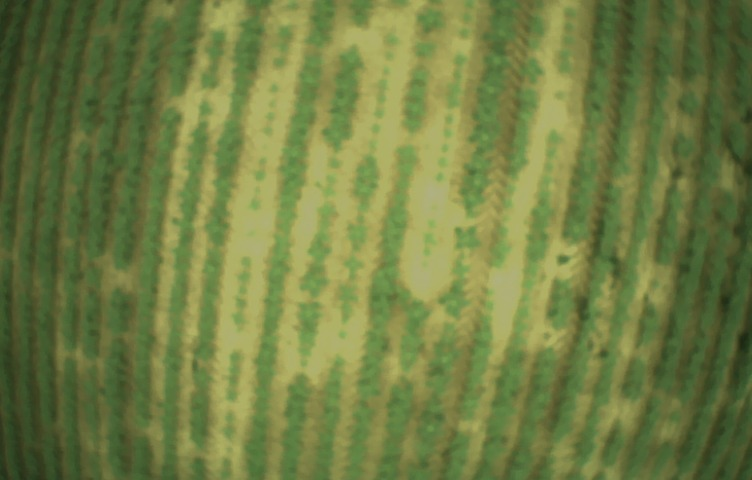
\includegraphics[width=80mm]{im30.jpg}}
  \caption{Sample CaspaPX images}
  \label{fig:caspa_sample}
\end{figure} 

\section{Time Synchronization of Sensors}
 
Currently there is loose time synchronization based on timestamps added to the scan and INS data streams at the application level. Tighter synchronization is planned in the future by time stamping at a lower level (i.e. in the device drivers) and by hardware sync between the scanner and the camera. The pulse output generated by the scanner at the start of each revolution could be used to trigger the exposure of a camera frame using it's exposure input. This input will be available on the custom camera design currently in development at the LAAS.

\section{Challenge Summary}

The section below summarizes the problems relative to the current platform for it's intended goal of creating DTMs.

\begin{itemize}
 \item Limited LIDAR detection range.
 \item Limited LIDAR resolution between scan lines at high aircraft velocities.
 \item High CPU usage of LIDAR device driver and low throughput especially with intensity data.
 \item Maintaining constant Above-Ground-Level (AGL) altitude in varying terrain to stay within the 10-15 m LIDAR range.
 \item Accurate attitude and position estimates needed for accurate data correction and geo-referencing.
 \item Limited range on R/C Link (150 m max for low altitudes which is less than ideal).
 \item Limited autonomy due to limited battery capacity (10-12 minutes maximum).
 \item Limited capacity of autopilot to closely follow flight plan tracks (even straight lines) in fluctuating or high winds.
 \item Frequent hardware failures due to the low-cost nature of RC products. Servos often die unexpectedly, intermittent solder joints on IR sensors, etc.
\end{itemize}

\chapter{Conclusion}

During the course of the project, I built a UAV and a payload and developed all of the software tools to permit it to capture data in flight. I also implemented an extensive amount of software to communicate the data to ground robots and to visualize the data on screen to analyze it visually. I became intimately familiar with the laser scanner, the IMU, and the camera sensors and especially their limitations. I also worked extensively with embedded Linux and the gumstix OMAP platform, cross-compiling and debugging drivers and applications in a variery of build environments. Finally, while I was already familiar with paparazzi, I learned more in aircraft configuration and tuning.

The hardware construction involved precise mechanical construction and electrical wiring, and took considerable time to do so that an easy-to-use, strong, compact, and light-weight system would result. These were the real-world constraints of an embedded and aeronautical system, and I am quite satisfied with the result.

This project showed that it is possible to fly the requested sensors on an autonomous aircraft. Through our 17 test flights we established that the AUV could follow our flight plans and that the lidar was capable of scanning the terrain in daylight conditions. This data could be recorded along with relatively accurate attitude and position estimates, we also successfully acquired camera imagery, and the ground communication links gave with positive results.

Unfortunately, the limited range of the laser scanner and autonomy of the aircraft render the UAV useful for only a few potential scenarios. The craft must fly very low to stay in scanner range so the environment to be scanned must not have elevations that vary more than a few meters and obstacles must also be only a few meters in size (no trees or buildings). This lends itself well in looking for ditches and roads in a typical desert or agricultural landscapes, but not at all for wooded or urban environments.

This was an ambitious project since it involved both the creation of a flying robot and the development of software to treat the resulting scientific data from a multitude of sensors. We were confronted with host of diverse practical issues and we managed to resolve them or work around them in the end. Other issues, like the very limited real-world range of the hokuyo is not something we can improve and the project, should it continue will need to fly the UAV at night, or use a different aircraft, or wait until an improved scanner is available.

\section{Concepts and Skills Learned}

Having never worked with cameras in detail and 3D modeling, I had the opportunity to enter a whole new world. I became familiar with openGL and representing 3D objects on screen, along with the coordinate transformations required to represent points acquired in a sensor reference frame in a global or ``world'' frame. I worked a little bit with the LAAS openrobots system but did not enter into as much depth there as I would have liked. I also touched on pin-hole camera models, and the methods and challenges related to the use of cameras in mapping an environment. On the more-practical side, I learned in detail camera interfacing details, both parallel as with the Caspa PX, but also the serial MIPI standards available on the OMAP processors. I had the pleasure of assisting an IUT intern in discovering the complex world of embedded processor development, and after he ramped up, he in turn showed me a few new things like kgdb kernel debugging.

\section{Thoughts on Future Direction}

By using the laser data to regulate the aircraft's altitude, it would be possible to follow gently changing terrain elevations. Another possibility worth investigation is the deflection of part or parts of the hokuyo's 270 degree scanning range towards the front of the aircraft. These scan portions could be used to detect obstacles and instruct the autopilot to fly over or around them, although the limited lidar range and high aircraft velocities would seriously limit this capability.

By using a different lidar scanner or improving the current driver performance, it would also be interesting to be able to receive intensity and multi-echo data. This data is useful for constructing terrain models in the presence of trees with leaves, for example.

Finally, due to the effective 10m lidar range, to stay safely above the terrain and achieve higher scan density, moving to either a slow flying airplane (5-7 m/s) or a quadrotor is required. Designs for these types of craft with payload capacity in the 700 gram range could be constructed at minimal cost. 

I investigated the design of slow-flying plane for our payload size with a drone aerodynamics PhD candidate from ENAC. We established the basic details and a hollow wing cross-section design to be cut from EPP foam, reinforced with carbon fiber tubing, and covered with smooth tape for strength and laminar air flow considerations. The aircraft would have a 2m wingspan, with removable wings and horizontal stabilizer for easy storage and transport. It would have an autonomy around 40 to 45 minutes when flying level at a speed of 5 m/s and providing 10W to the payload electronics. Higher speed flight is possible but at 10 m/s the autonomy reduces to less than 20 minutes. This platform goes a long way in addressing many of the drawbacks of our payload sensors and promises more complete and interesting data than our current mentor-based platform. Initial drawings are shown in Figure \ref{fig:murat_design}.

\begin{figure}[ht]
  \centering
  \subfloat[Plan View]{\label{fig:murat1}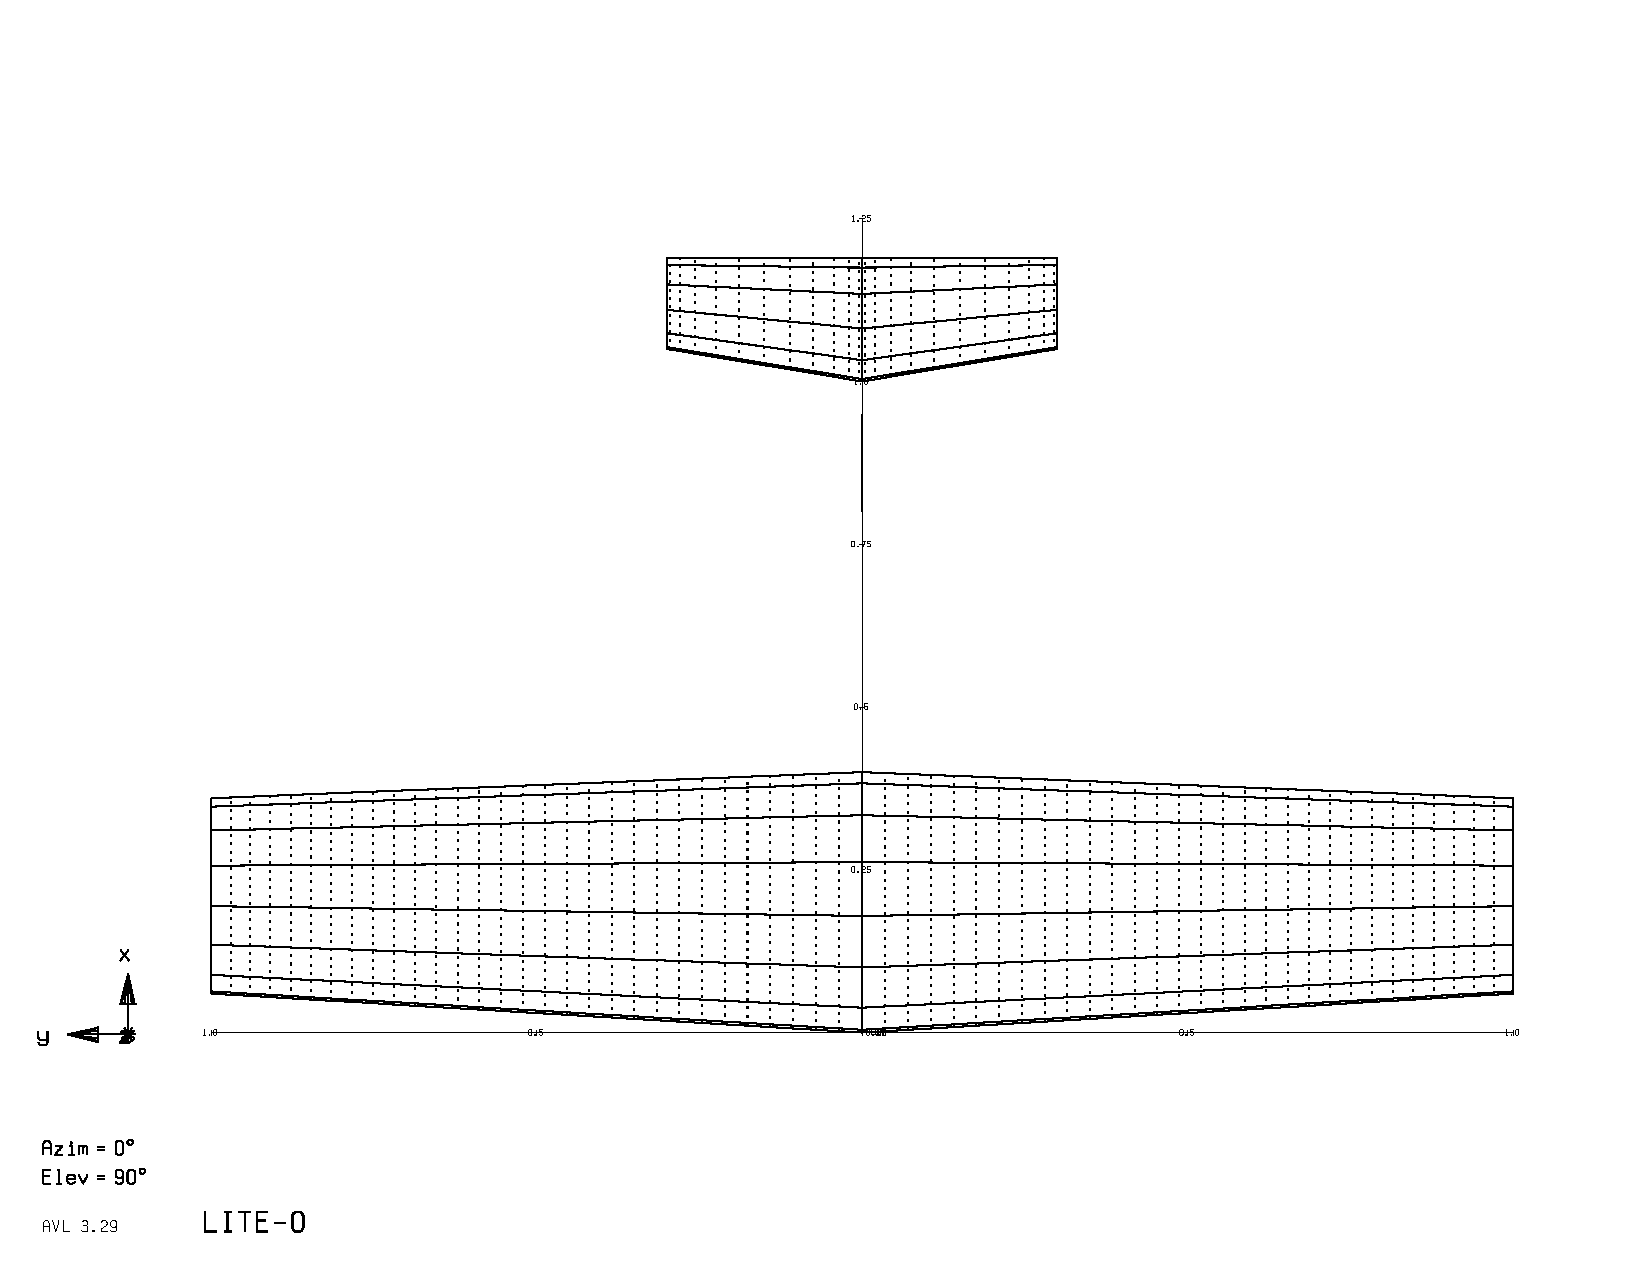
\includegraphics[width=80mm]{murat1}}                
  \subfloat[Isometric View]{\label{fig:murat2}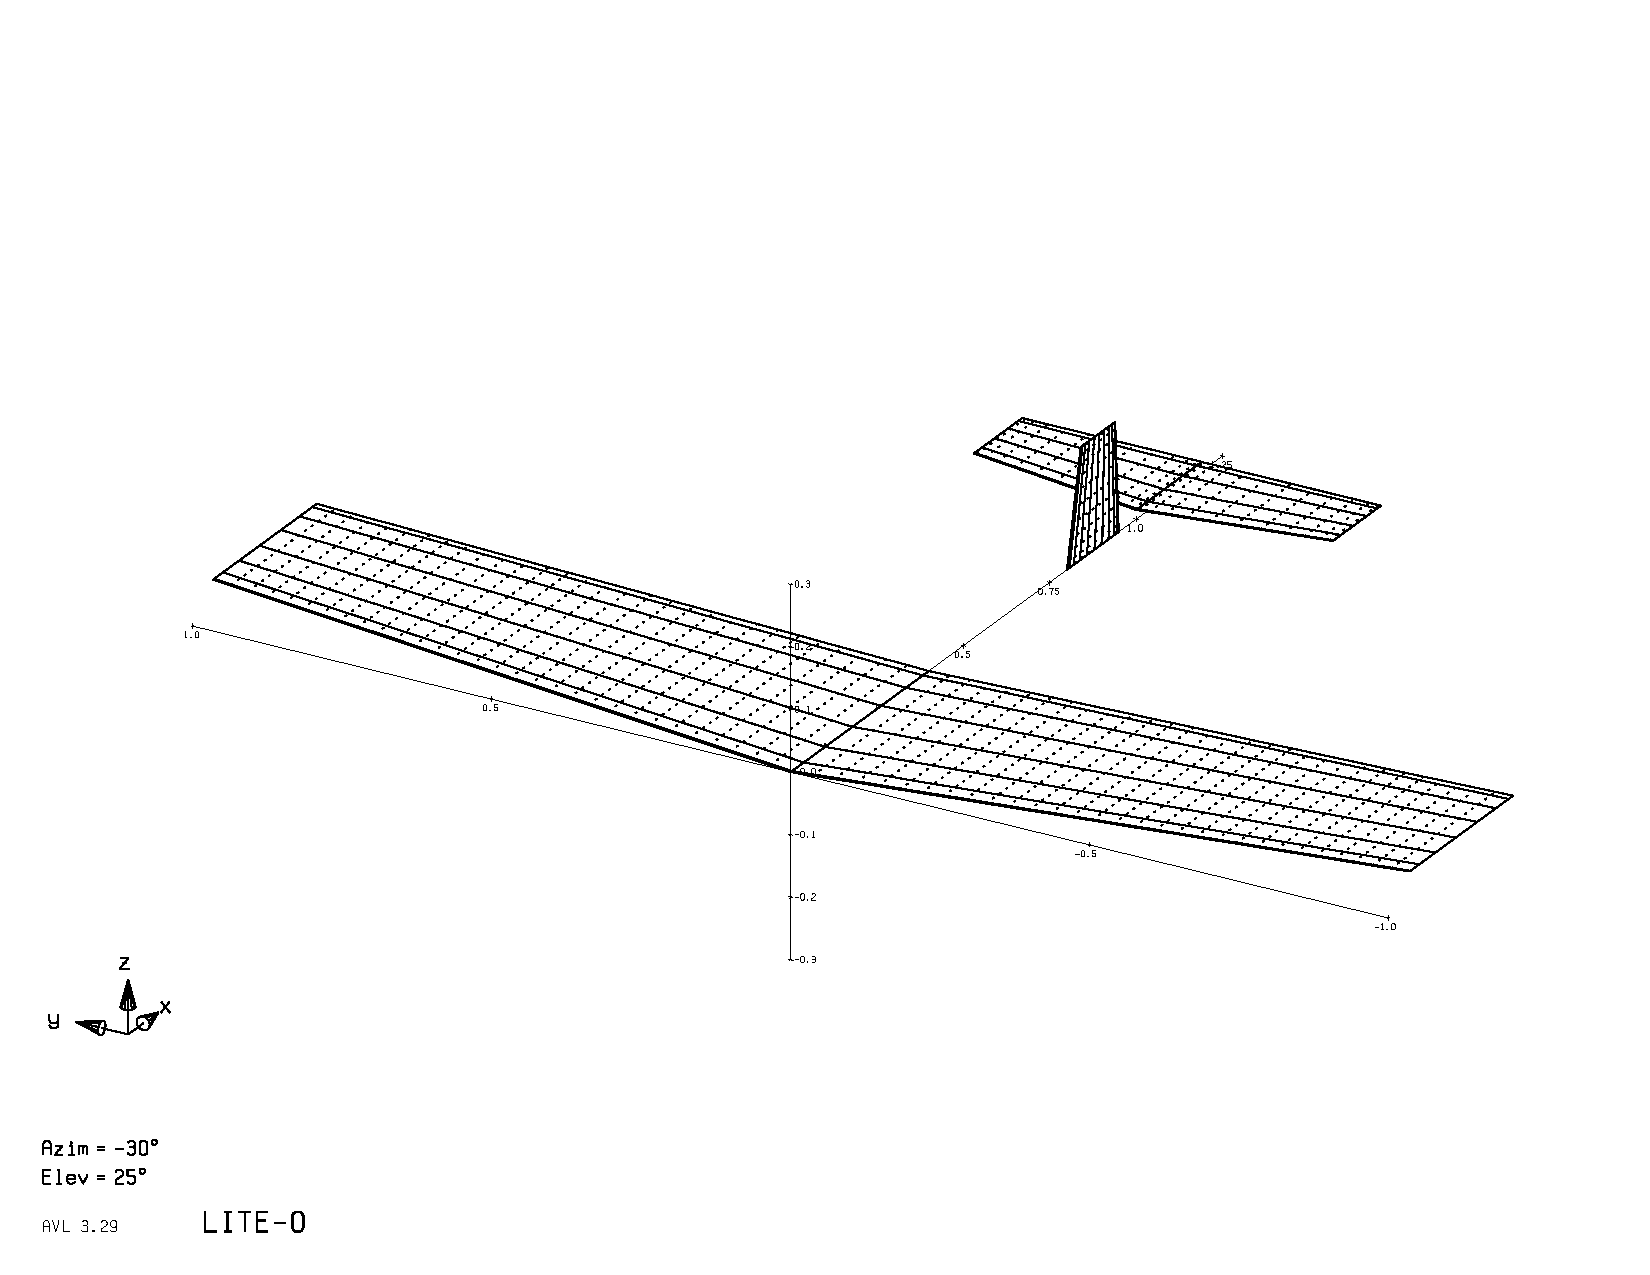
\includegraphics[width=80mm]{murat2}}
  \caption{Slow Flyer Design Concept}
  \label{fig:murat_design}
\end{figure} 

The other alternative is to use a quadrotor such as the Asctec platform recently acquired by the LAAS (Figure \ref{fig:quad}). While autonomy and range are less than for fixed-wing platforms they can remain stationary or move very slowly and can be used or at least tested indoors. These advantages are the reason why this sort of craft is fairly common and found in many labs around the world.

\begin{figure}[ht]
  \centering
  \subfloat[With low-cost Hokuyo device]{\label{fig:asctec1}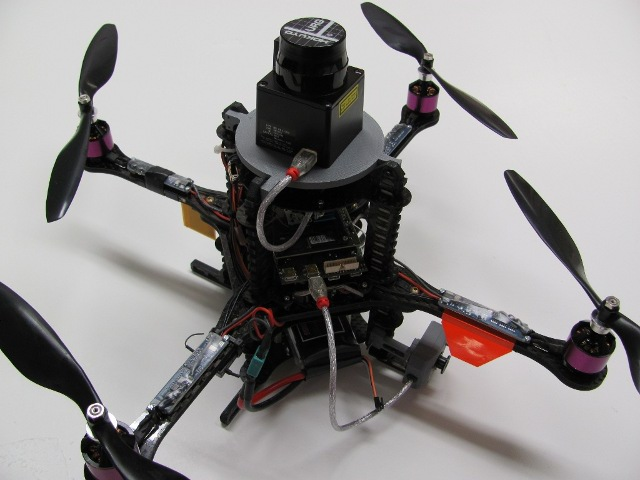
\includegraphics[width=80mm]{asctec1.jpg}}                
  \subfloat[With UTM30-LX]{\label{fig:asctec2}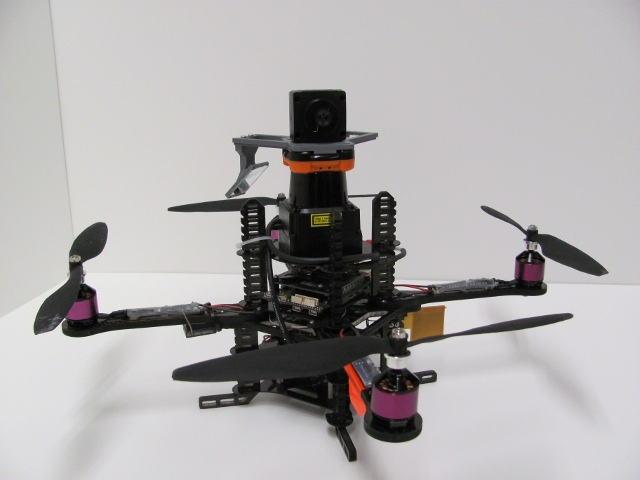
\includegraphics[width=80mm]{asctec2.jpg}}
  \caption{Asctec Quad-rotor platform}
  \label{fig:quad}
\end{figure} 

\section{Acknowledgments}

I thank my mentor Bertrand Vandeportaele for his constant involvement and willingness to explain new subjects to me. I must also recognize the members of the ENAC drone lab, especially Gautier Hattenberger, Michel Gorraz, and Antoine Drouin, as being very helpful and key in the success of the build. They provided space, tools, equipment, and materials for construction, along with a healthy number of ideas to solve the various practical challenges encountered along the way.

\begin{thebibliography}{9}

\bibitem{ugvs}
  \url{http://homepages.laas.fr/matthieu/robots/}

%http://spiderman-2.laas.fr/robots/index.php

\bibitem{rackham}
  \url{http://homepages.laas.fr/sara/robots/rackham/index.php}

\bibitem{jido}
  \url{http://homepages.laas.fr/matthieu/robots/jido.shtml}

\bibitem{dala}
  \url{http://homepages.laas.fr/sara/robots/dala/index.php}

\bibitem{this}
  \url{http://paparazzi.enac.fr/wiki/Laserhawk}

\bibitem{karma}
  \url{http://homepages.laas.fr/matthieu/robots/karma.shtml}

\bibitem{lhassa}
  \url{http://homepages.laas.fr/sara/robots/lhassa/index.php}

\bibitem{gautier}
  Gautier Hattenberger,
  \emph{Formation flight: evaluation of autonomous configuration control algorithms}.
  \url{homepages.laas.fr/simon/publis/HATTENBERGER-IAV-2007.pdf}
  Intelligent Robots and Systems, 2007. IROS 2007. IEEE/RSJ International Conference, 
  2007.

\bibitem{manta}
  \url{http://homepages.laas.fr/bvandepo/wiki/doku.php?id=descriptionmanta}

\bibitem{caspa}
  \url{http://wiki.gumstix.org/index.php?title=Caspa_camera_boards}

\bibitem{robotpkg}
  \url{http://www.openrobots.org/wiki}

\bibitem{laserhawkgit}
  \url{https://github.com/paulcox/laserhawk}

\bibitem{paparazzi}
  \url{http://paparazzi.enac.fr/wiki/Main_Page}

\bibitem{elrob}
  \url{http://www.elrob.org/}

\bibitem{omap}
  \url{processors.wiki.ti.com/index.php/OMAP3_Overview}

\bibitem{Overo}
  \url{http://www.gumstix.com/store/catalog/product_info.php?products_id=211}

\bibitem{asctec}
  \url{http://www.asctec.de/home-en}

\bibitem{multiplex}
  \url{http://www.multiplexusa.com/}

\bibitem{murat}
  Murat Bronz, Jean Marc Moschetta, Pascal Brisset, Michel Gorraz
  \emph{Towards a Long Endurance MAV}
  \url{http://www.recherche.enac.fr/LOTA/lib/exe/fetch.php?id=pascal_brisset&cache=cache&media=03-bronz_moschetta_ijmav.pdf}
  \url{www.emav09.org/EMAV-final-papers/paper_78.pdf}
  International Journal of Micro Air Vehicles
  Volume 1 · Number 4 · December 2009

\bibitem{corsica}
  \url{http://paparazzi.enac.fr/wiki/Corsica}

\bibitem{paparazzi_paper}
  Pascal Brisset, Antoine Drouin, Michel Gorraz, Pierre-Selim Huard and Jeremy Tyler
  \emph{The Paparazzi Solution}
  \url{http://www.recherche.enac.fr/paparazzi/papers_2006/mav06_paparazzi.pdf}
  MAV '06,
  October 2006

\bibitem{norman_paper}
 Juchler, Norman
 \emph{Homography-based Method To Generate A Traversability Map Using Aerial Images}
 LAAS-CNRS Master Thesis,
 April 27, 2009

\bibitem{redouane_paper}
 Redouane Boumghar, and Simon Lacroix, Olivier Levebvre
 \emph{An Information-Driven Navigation Strategy for Autonomous Rover Navigation in Unknown Environments}
 LAAS-CNRS
 May 2011

\end{thebibliography}

\appendix
\appendixpage
\addappheadtotoc

\chapter{Airframe Configuration}

\definecolor{listinggray}{gray}{0.9}
\definecolor{lbcolor}{rgb}{0.9,0.9,0.9}

\lstset{
  basicstyle=40pt,       % the size of the fonts that are used for the code
  numbersep=25pt,
  numbers=left,
  backgroundcolor=\color{lbcolor},
  tabsize=4,
  rulecolor=,
  language=XML,
  basicstyle=\scriptsize,
  upquote=true,
  aboveskip={1.5\baselineskip},
  columns=fixed,
  showstringspaces=false,
  extendedchars=true,
  breaklines=true,
  prebreak = \raisebox{0ex}[0ex][0ex]{\ensuremath{\hookleftarrow}},
  frame=single,
  showtabs=false,
  showspaces=false,
  showstringspaces=false,
  identifierstyle=\ttfamily,
  keywordstyle=\color[rgb]{0,0,1},
  commentstyle=\color[rgb]{0.133,0.545,0.133},
  stringstyle=\color[rgb]{0.627,0.126,0.941},
}

\lstset{caption=Airframe Configuration}

\begin{lstlisting}
<!DOCTYPE airframe SYSTEM "../airframe.dtd">


<airframe name="Mentor Laas N1 Tiny 1.1">


  <firmware name="fixedwing">
    <target name="sim" 			board="pc">
      <define name="AGR_CLIMB" />
      <define name="LOITER_TRIM" />
      <define name="ALT_KALMAN" />
    </target>
    <target name="ap" 			board="tiny_1.1">
      <define name="AGR_CLIMB" />
      <define name="LOITER_TRIM" />
      <define name="ALT_KALMAN" />
    </target>

    <subsystem name="radio_control" type="ppm"/>

    <!-- Communication -->
    <subsystem name="telemetry" 	type="transparent">
      <configure name="MODEM_BAUD" 		value="B57600"/>
    </subsystem>

    <subsystem name="control"/>
    <!-- Sensors -->
    <subsystem name="attitude" 		type="infrared">
      <configure name="ADC_IR1" value="ADC_1"/>
      <configure name="ADC_IR2" value="ADC_0"/>
      <configure name="ADC_IR_TOP" value="ADC_3"/>
    </subsystem>
    <subsystem name="gps" 		    type="ublox_lea4p"/>
    <subsystem name="navigation"/>

  </firmware>

  <firmware name="setup">
    <target name="tunnel"           board="tiny_1.1" />
    <target name="setup_actuators"  board="tiny_1.1" />
  </firmware>

  <modules>
    <load name="cartography.xml"/>
    <load name="adc_generic.xml">
      <configure name="ADC_CHANNEL_GENERIC1" value="ADC_2"/>
      <configure name="ADC_CHANNEL_GENERIC2" value="ADC_4"/>
    </load>
  </modules>

<!-- commands section -->
  <servos>
    <servo name="THROTTLE"   no="0" min="1200" neutral="1200" max="2000"/>
    <servo name="AILERON_LEFT"  no="3" min="1900" neutral="1550" max="1100"/>
    <servo name="AILERON_RIGHT" no="1" min="1900" neutral="1520" max="1100"/>
    <servo name="RUDDER" no="4" min="1850" neutral="1500" max="1150"/>
    <servo name="ELEVATOR" no="5" min="2200" neutral="1400" max="1000"/>
  </servos>

  <commands>
    <axis name="THROTTLE" failsafe_value="0"/>
    <axis name="ROLL"     failsafe_value="0"/>
    <axis name="PITCH"    failsafe_value="0"/>
    <axis name="YAW"      failsafe_value="0"/>
  </commands>

  <rc_commands>
    <set command="THROTTLE" value="@THROTTLE"/>
    <set command="ROLL"     value="@ROLL"/>
    <set command="PITCH"    value="@PITCH"/>
    <set command="YAW"    value="@YAW"/>
  </rc_commands>

  <section name="MIXER">
    <define name="AILERON_DIFF" value="0.66"/>
    <define name="COMBI_SWITCH" value="1.0"/>
  </section>

  <command_laws>
    <set servo="THROTTLE"           value="@THROTTLE"/>
    <set servo="ELEVATOR" value="@PITCH"/>
    <set servo="RUDDER" value="@YAW + @ROLL*COMBI_SWITCH"/>

    <let var="roll" value="@ROLL"/>
    <set servo="AILERON_LEFT" value="($roll > 0 ? 1 : AILERON_DIFF) * $roll"/>
    <set servo="AILERON_RIGHT" value="($roll > 0 ? AILERON_DIFF : 1) * $roll"/>
  </command_laws>

  <section name="AUTO1" prefix="AUTO1_">
    <define name="MAX_ROLL" value="0.6"/>
    <define name="MAX_PITCH" value="0.6"/>
  </section>

  <section name="INFRARED" prefix="IR_">
    <define name="ROLL_NEUTRAL_DEFAULT" value="-2.6" unit="deg"/>
    <define name="PITCH_NEUTRAL_DEFAULT" value="0.6" unit="deg"/>

    <define name="HORIZ_SENSOR_TILTED" value="1"/>
    <define name="IR2_SIGN" value="-1"/>
    <define name="TOP_SIGN" value="-1"/>

    <!--linear name="RollOfIrs" arity="2" coeff1="0.7" coeff2="0.7"/>
    <linear name="PitchOfIrs" arity="2" coeff1="-0.7" coeff2="0.7"/>
    <linear name="TopOfIr" arity="1" coeff1="1.5"/-->

    <define name="ADC_IR1_NEUTRAL" value="507"/>
    <define name="ADC_IR2_NEUTRAL" value="509"/>
    <define name="ADC_TOP_NEUTRAL" value="515"/>

    <define name="LATERAL_CORRECTION" value="1."/>
    <define name="LONGITUDINAL_CORRECTION" value="1."/>
    <define name="VERTICAL_CORRECTION" value="1."/>
  </section>

  <section name="BAT">
    <define name="MILLIAMP_AT_FULL_THROTTLE" value="40000"/>
    <define name="CATASTROPHIC_BAT_LEVEL" value="9.3" unit="V"/>
  </section>

  <section name="MISC">
    <define name="NOMINAL_AIRSPEED" value="18." unit="m/s"/>
    <define name="MINIMUM_AIRSPEED" value="11." unit="m/s"/>
    <define name="MAXIMUM_AIRSPEED" value="33." unit="m/s"/>
    <define name="CARROT" value="3." unit="s"/>
    <define name="KILL_MODE_DISTANCE" value="(1.5*MAX_DIST_FROM_HOME)"/>
<!--    <define name="XBEE_INIT" value="\"ATPL2\rATRN1\rATTT80\rATBD6\rATWR\r\""/> -->
    <define name="XBEE_INIT" value="\"ATPL2\rATRN1\rATTT80\r\""/>
<!--    <define name="NO_XBEE_API_INIT" value="TRUE"/> -->
    <define name="ALT_KALMAN_ENABLED" value="TRUE"/>
    <define name="TRIGGER_DELAY" value="1."/>
    <define name="DEFAULT_CIRCLE_RADIUS" value="80."/>
  </section>

  <section name="VERTICAL CONTROL" prefix="V_CTL_">

    <define name="POWER_CTL_BAT_NOMINAL" value="11.1" unit="volt"/>
    <!-- outer loop proportional gain -->
    <define name="ALTITUDE_PGAIN" value="-0.15"/>
    <!-- outer loop saturation -->
    <define name="ALTITUDE_MAX_CLIMB" value="2."/>

    <!-- auto throttle inner loop -->
    <define name="AUTO_THROTTLE_NOMINAL_CRUISE_THROTTLE" value="0.55"/>
    <define name="AUTO_THROTTLE_MIN_CRUISE_THROTTLE" value="0.30"/>
    <define name="AUTO_THROTTLE_MAX_CRUISE_THROTTLE" value="0.90"/>
    <define name="AUTO_THROTTLE_LOITER_TRIM" value="0"/>
    <define name="AUTO_THROTTLE_DASH_TRIM" value="0"/>
    <define name="AUTO_THROTTLE_CLIMB_THROTTLE_INCREMENT" value="0.05" unit="%/(m/s)"/>
    <define name="AUTO_THROTTLE_PGAIN" value="-0.03"/>
    <define name="AUTO_THROTTLE_IGAIN" value="0.05"/>
    <define name="AUTO_THROTTLE_PITCH_OF_VZ_PGAIN" value="0.03"/>
    
    <!-- auto pitch inner loop -->
    <define name="AUTO_PITCH_PGAIN" value="-0.065"/>
    <define name="AUTO_PITCH_IGAIN" value="0.15"/>
    <define name="AUTO_PITCH_MAX_PITCH" value="0.35"/>
    <define name="AUTO_PITCH_MIN_PITCH" value="-0.35"/>

    <define name="THROTTLE_SLEW" value="0.05"/>

  </section>

  <section name="HORIZONTAL CONTROL" prefix="H_CTL_">
    <define name="COURSE_PGAIN" value="-1."/>
    <define name="ROLL_MAX_SETPOINT" value="0.6" unit="radians"/>
    <define name="PITCH_MAX_SETPOINT" value="0.5" unit="radians"/>
    <define name="PITCH_MIN_SETPOINT" value="-0.5" unit="radians"/>


    <define name="ROLL_ATTITUDE_GAIN" value="-10000"/>
    <define name="AILERON_OF_THROTTLE" value="0.0"/>
    <define name="PITCH_PGAIN" value="-12000."/>
    <define name="PITCH_DGAIN" value="1.5"/>
    <define name="ELEVATOR_OF_ROLL" value="1250"/>
  </section>

  <section name="NAV">
    <define name="NAV_PITCH" value="0."/>
    <define name="NAV_GLIDE_PITCH_TRIM" value="0"/>
    <define name="NAV_GROUND_SPEED_PGAIN" value="-0.015"/>
    <define name="NAV_FOLLOW_PGAIN" value="-0.05"/>
  </section>

  <section name="FORMATION" prefix="FORM_">
    <define name="CARROT" value="3." unit="s"/> <!-- carrot distance for followers -->
    <define name="POS_PGAIN" value="0.02"/> <!-- coef on position error -->
    <define name="SPEED_PGAIN" value="0.4"/> <!-- coef on speed error -->
    <define name="COURSE_PGAIN" value="0.8"/> <!-- coef on course error (override course pgain for followers) -->
    <define name="ALTITUDE_PGAIN" value="0.1"/> <!-- coef on altitude error -->
    <define name="PROX" value="60." unit="m"/> <!-- proximity distance -->
    <define name="MODE" value="0"/> <!-- mode 0 = global, 1 = local -->
  </section>

  <section name="TCAS" prefix="TCAS_">
    <define name="TAU_TA" value="10." unit="s"/> <!-- traffic advisory -->
    <define name="TAU_RA" value="6." unit="s"/> <!-- resolution advisory -->
    <define name="ALIM" value="15." unit="m"/> <!-- altitude limitation -->
    <define name="DT_MAX" value="2000" unit="ms"/> <!-- lost comm or timeout -->
  </section>

  <section name="POTENTIAL">
    <define name="FORCE_POS_GAIN" value="50"/>
    <define name="FORCE_SPEED_GAIN" value="1"/>
    <define name="FORCE_CLIMB_GAIN" value="8"/>
  </section>

  <section name="AGGRESSIVE" prefix="AGR_">
    <define name="BLEND_START" value="20"/><!-- Altitude Error to Initiate Aggressive Climb CANNOT BE ZERO!!-->
    <define name="BLEND_END" value="10"/><!-- Altitude Error to Blend Aggressive to Regular Climb Modes  CANNOT BE ZERO!!-->
    <define name="CLIMB_THROTTLE" value="0.8"/><!-- Gaz for Aggressive Climb -->
    <define name="CLIMB_PITCH" value="0.3"/><!-- Pitch for Aggressive Climb -->
    <define name="DESCENT_THROTTLE" value="0.1"/><!-- Gaz for Aggressive Decent -->
    <define name="DESCENT_PITCH" value="-0.25"/><!-- Pitch for Aggressive Decent -->
    <define name="CLIMB_NAV_RATIO" value="0.8"/><!-- Percent Navigation for Altitude Error Equal to Start Altitude -->
    <define name="DESCENT_NAV_RATIO" value="1.0"/>
  </section>

  <section name="FAILSAFE" prefix="FAILSAFE_">
    <define name="DELAY_WITHOUT_GPS" value="1" unit="s"/>
    <define name="DEFAULT_THROTTLE" value="0.3" unit="%"/>
    <define name="DEFAULT_ROLL" value="0.3" unit="rad"/>
    <define name="DEFAULT_PITCH" value="0.5" unit="rad"/>
    <define name="HOME_RADIUS" value="100" unit="m"/>
  </section>

  <section name="SIMU">
    <define name="YAW_RESPONSE_FACTOR" value="1."/>
  </section>

 <makefile>

  </makefile>
</airframe>
\end{lstlisting}

\chapter{Code Listings}

\lstset{
  basicstyle=40pt,       % the size of the fonts that are used for the code
  numbersep=25pt,
  numbers=left,
  backgroundcolor=\color{lbcolor},
  tabsize=4,
  rulecolor=,
  language=PERL,
  basicstyle=\scriptsize,
  upquote=true,
  aboveskip={1.5\baselineskip},
  columns=fixed,
  showstringspaces=false,
  extendedchars=true,
  breaklines=true,
  prebreak = \raisebox{0ex}[0ex][0ex]{\ensuremath{\hookleftarrow}},
  frame=single,
  showtabs=false,
  showspaces=false,
  showstringspaces=false,
  identifierstyle=\ttfamily,
  keywordstyle=\color[rgb]{0,0,1},
  commentstyle=\color[rgb]{0.133,0.545,0.133},
  stringstyle=\color[rgb]{0.627,0.126,0.941},
}

\lstset{caption=}

\section{mkvirtlog.pl}
\lstinputlisting[]{../log2gdhe/mkvirtlog.pl}
\section{mkvirts.pl}
\lstinputlisting[]{../log2gdhe/mkvirts.pl}
\section{plotlogs.pl}
\lstinputlisting[]{../biketest/scripts/plotlogs.pl}
\section{animatelogs.pl}
\lstinputlisting[]{../biketest/scripts/animatelogs.pl}
\section{getmaps.pl}
\lstinputlisting[]{../biketest/scripts/getmaps.pl}
\section{gmaps.pl}
\lstinputlisting[]{../biketest/scripts/utils/gmaps.pl}
\section{hokumti.pl}
This Perl script runs on the airborne target and uses an early version of the getrange executable to obtain the hokuyo range data and the MTIHardTest executable to obtain the MTI data. Due to high CPU utilization, it was abandoned for the getrange program below which does all data acquisition and logging from within a single application/thread.
\lstinputlisting[]{../biketest/scripts/utils/hokumti.pl}

\lstset{language=C++}
\section{getrange C++ program}
This program runs on the omap target and is responsible for gathering all sensor data, logging it, and sending it to the ground.
\lstinputlisting[]{../../bvdp_pprz/sw/airborne/firmwares/laserhawk/main.cpp}

\lstset{language=make}
\section{Laserhawk.xml}
This is the makefile used to compile getrange.c

To compile the application, use the following paparazzi build command : 

make AIRCRAFT=LASERHAWK getrange.compile

\lstinputlisting[]{../../bvdp_pprz/conf/airframes/LAAS/laserhawk.xml}

\end{document}          
